\chapter{Results} \label{chap:results}
\section{Validation and Verification}
Validation and Verification (V\&V) are needed to make sure that our code works as we suppose. It is a necessary process in the field of computational simulations. They are essential for ensuring the reliability and accuracy of simulation model. Verification is the process of confirming that a computational model accurately implements the intended mathematical model or theory. It checks that the simulation does what it's supposed to do mathematically and computationally.
It involves code verification (checking the code's or algorithm's accuracy) and solution verification (ensuring the solution is numerically accurate). Standard practices include checking against analytical solutions, performing grid convergence studies, and conducting code-to-code comparisons.
Validation is the process of determining how well a computational model represents the real world. It is about assessing the accuracy of the simulation results in capturing the physical phenomena being modeled.

This involves comparing simulation results with experimental or real-world data. It can include sensitivity analyses, uncertainty quantification, and benchmark cases. The aim is to demonstrate that the model can produce sufficiently accurate results for its intended application, ensuring the model's credibility in representing physical reality.

For complex simulations, such as turbulent flows or multi-physics problems, V\&V can be challenging due to the complexity of the phenomena and the need for exact analytical solutions.

We conducted three experiments to confirm that the implemented solver operates as expected:
\begin{itemize}
    \item \textbf{A falling sphere example, 1 phase}. Experiment for one phase and one solid body, in our case it is sphere. 
    \item \textbf{A bouncing sphere example, water-air}. Experiment with two phases and one solid body. Density of the body smaller than one of the phase which make the body bounce and do not sink.
    \item \textbf{A falling multi-spherical body}. This will show that multi-spherical body in the shape of sphere act the same way as a simple sphere.
\end{itemize}

\subsection{A falling sphere example, 1 phase}
Based on the plan of initial validation of the created numerical model. We conducted a comparison between a one phase falling sphere simulation and the results presented in \cite{nan2023high}. The simulation utilized parameters for both the fluid and particle, which are provided in the {Table \ref{table1-chap4}}. Same simulation results provided in work \cite{nan2023high}, while Figure \ref{fig:1ph_exp_me} showcases the results work of the current solver. Based on a visual analysis, it is evident that the velocity of the fluid field around both particles is nearly identical. 

\begin{table}[H]
    \centering
    \caption{Simulation Parameters} \label{table1-chap4}
    \begin{tabular}{llr}
        \toprule
        \hline
        Simulation Part         & Physical Parameters (units) & Value \\
        \hline
        \midrule
        Particle                 & Density (kg/m$^3$)          & 1200    \\
                         & Diameter (cm)          & 0.167    \\
                         & Initial height (cm)          & 3.5    \\
                         \hline
        Fluid                  & Density (kg/m$^3$)           & 1000   \\
                                & Viscosity (m$^2$/s)         & 1e$^{-6}$    \\
                                \hline
        \bottomrule
     \end{tabular}
\end{table}
%
%\begin{figure}[!ht]
%    \centering
%    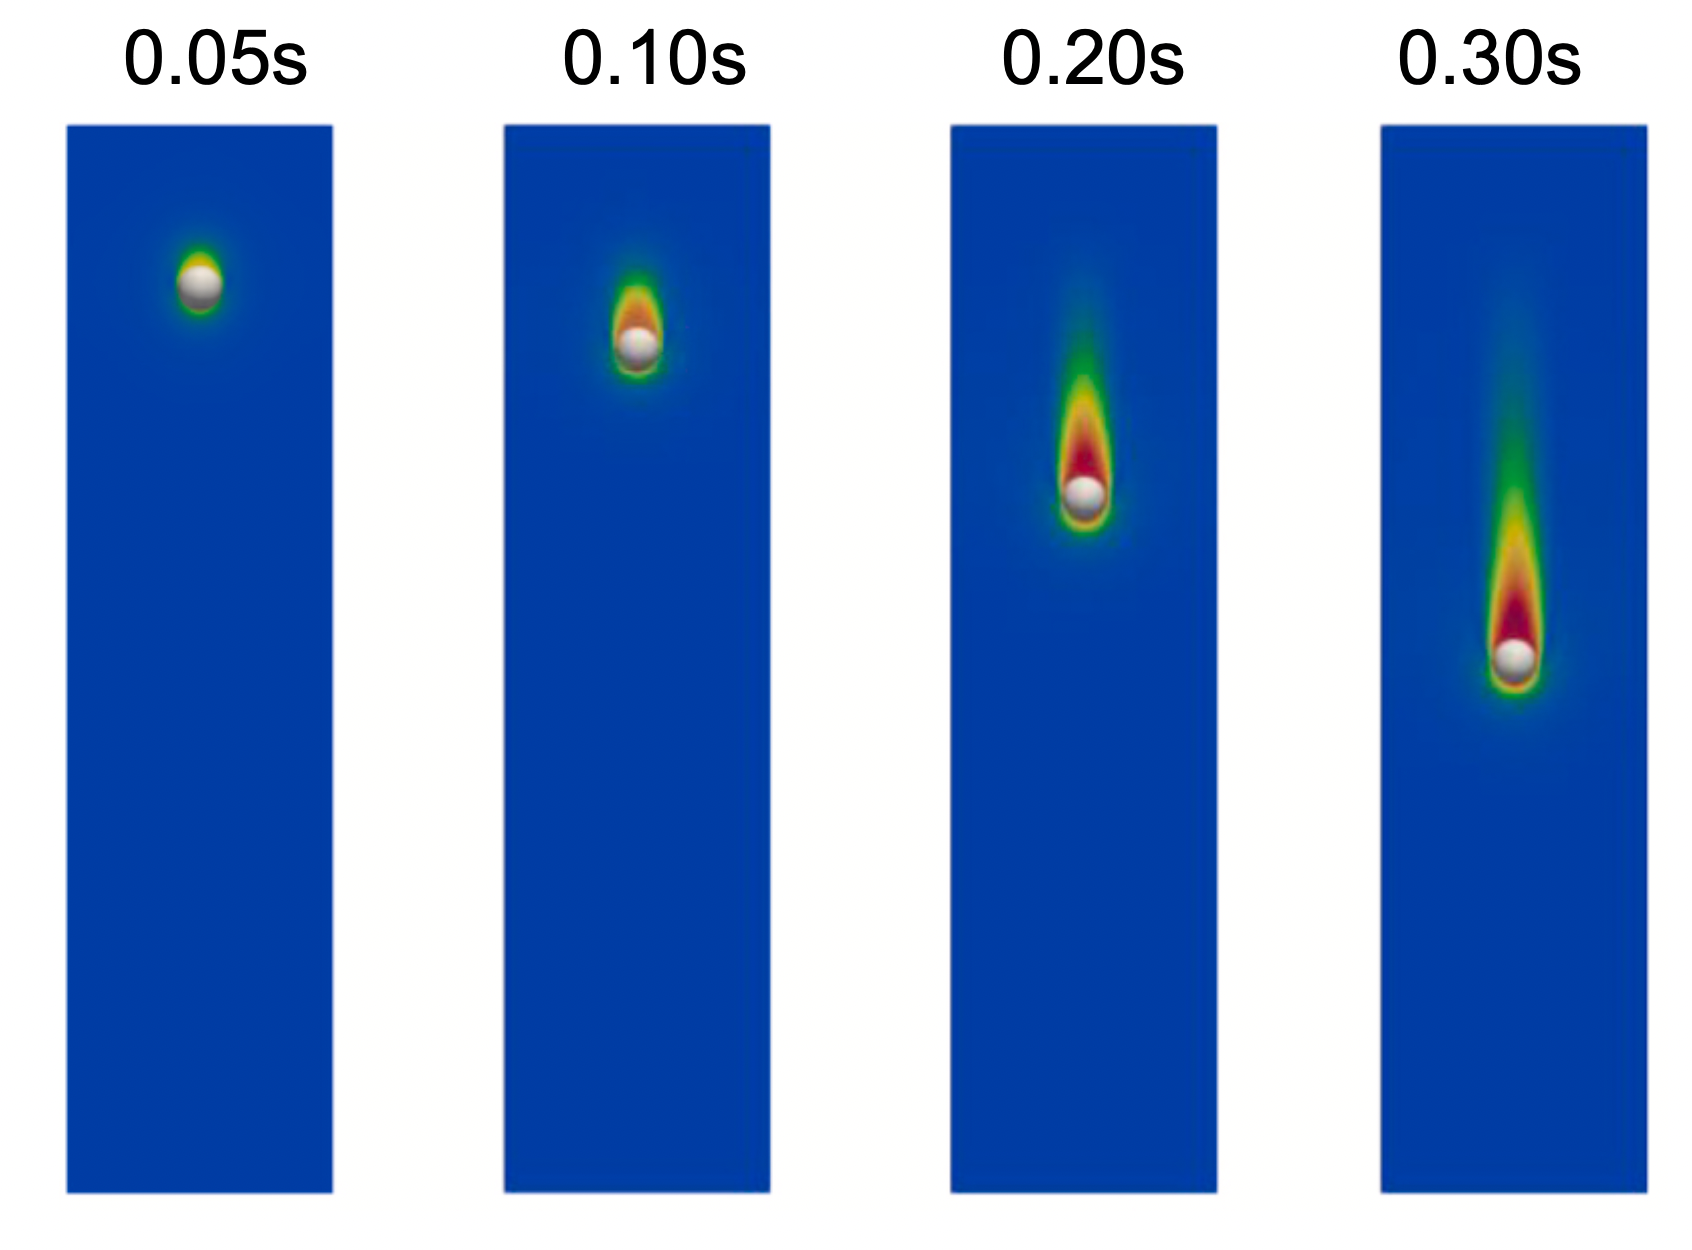
\includegraphics[width=10cm]{Images/chap3/1ph_exp.png}
%    \caption{Falling sphere simulation in 1 phase fluid from the work \cite{nan2023high}.}
%    \label{fig:1ph_exp}
%\end{figure}

\begin{figure}[!ht]
    \centering
    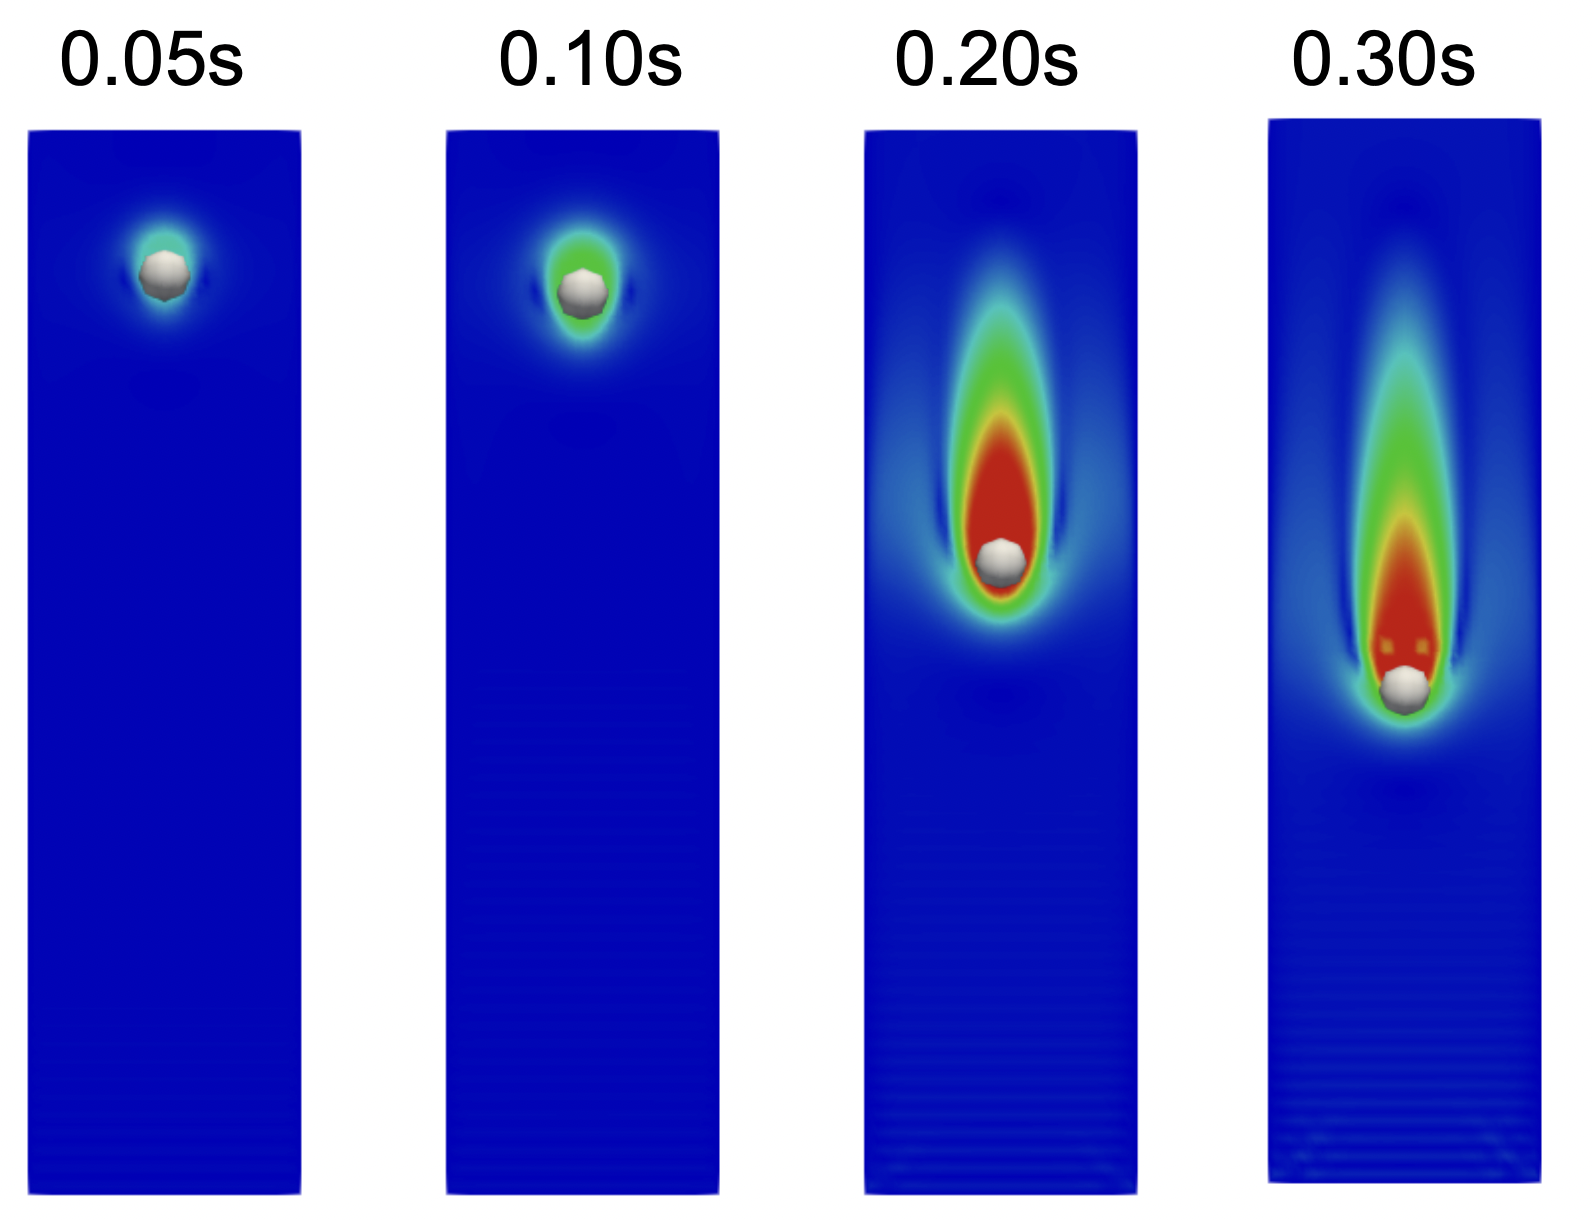
\includegraphics[width=10cm]{Images/chap3/1ph_exp_me.png}
    \caption{Velocity magnitude for falling sphere simulation in 1 phase fluid from the CFD-DEM simulation.}
    \label{fig:1ph_exp_me}
\end{figure}

More details are shown in Figure \ref{fig:trajectory_1ph}. The graph illustrates the trajectory and velocity comparison of a falling sphere in a one-phase fluid within our CFD-DEM simulation solver against the results published by Nan et al. (2023) \cite{nan2023high}. Both datasets present the time evolution of the sphere's $z$-direction movement and corresponding velocity. The plots are in good agreement with our simulation data (indicated by the orange dots) and the benchmark results from Nan et al. (2023)\cite{nan2023high} (represented by the solid black line) across the entirety of the simulated timeframe. This consistency in both position and velocity profiles supports solvers' ability to replicate particle motion dynamics within a fluid accurately. Minor variations observed are within acceptable ranges and may be attributed to the inherent discretization differences between the two simulation approaches. The coherence of the data underscores the reliability of our CFD-DEM simulation parameters and captures the essential physics of particle-fluid interaction.

\begin{figure}[!h]
    \centering
    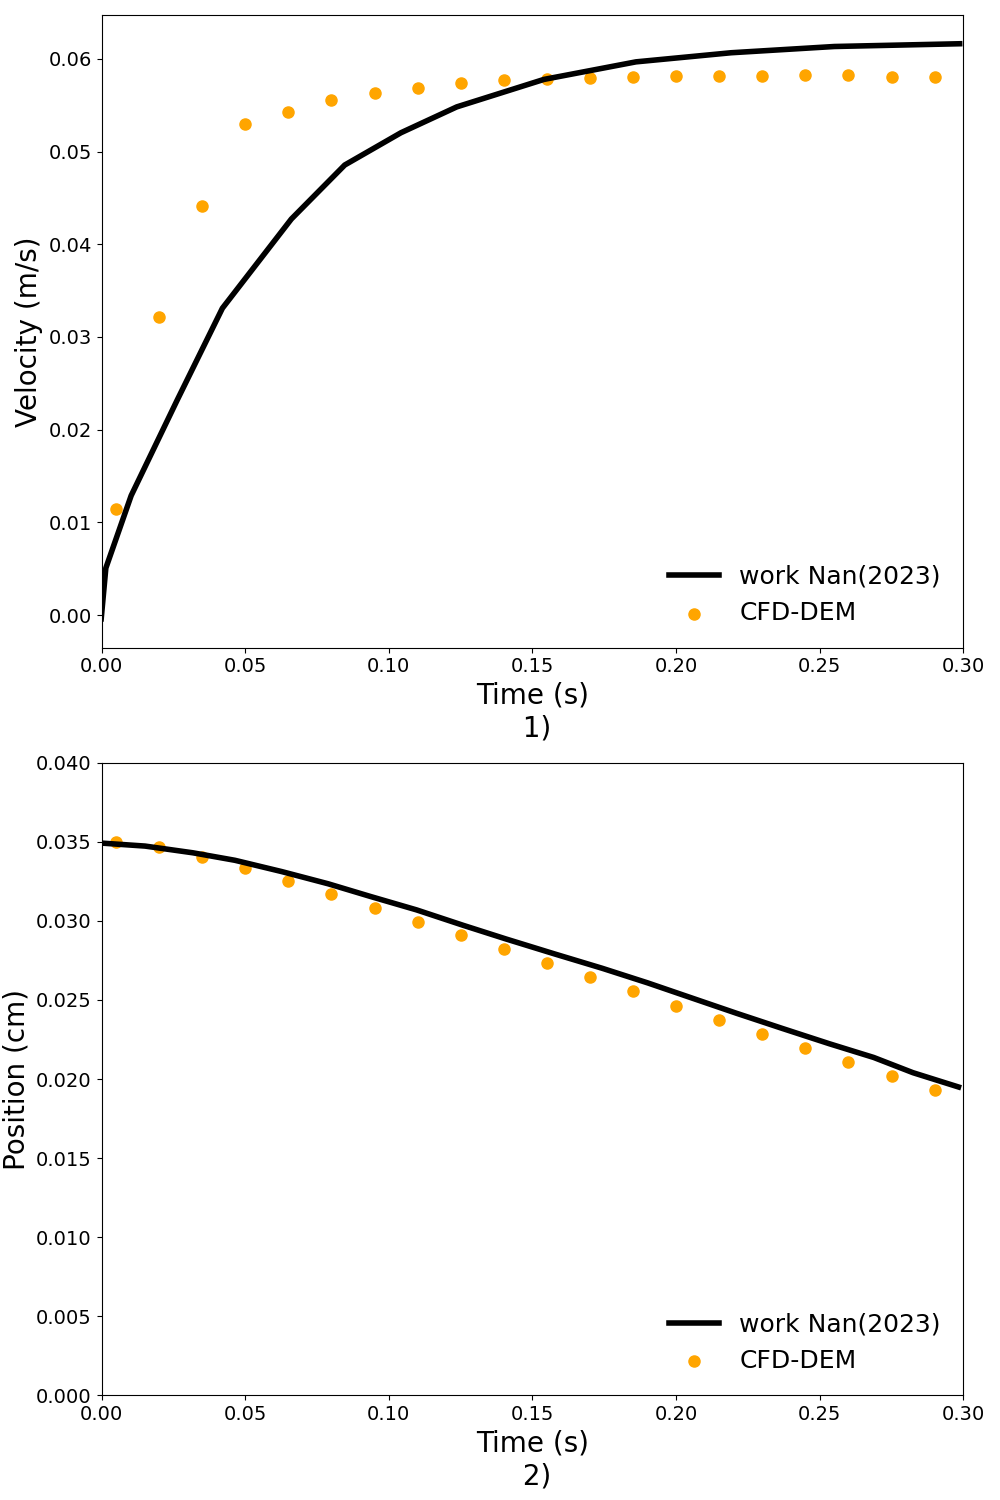
\includegraphics[width=13cm]{GWU_Thesis_Sarmakeeva/Images/chap3/nan_simulation_192000_cells_dt_0_0005_simulation.png}
    \caption{Falling sphere in 1 phase fluid 1) comparison in z-direction 2) velocity of the particle}
    \label{fig:trajectory_1ph}
\end{figure}

\newpage

\subsection{Grid convergence analysis.}

According to Roache's definition of code verification \cite{roache1998verification}, to confirm the ability to accurately solve the set of governing equations. A main strategy for validating the code is to convey a grid convergence study, which involves executing multiple simulations on successive finer grids. The discretization error is expected to approach zero asymptotically as the grid refined. The major point of interest in this context is the approximation order derived from the numerical method. For instance, if a second-order accurate method is used, it is reasonable to anticipate second-order convergence. However in most of the cases the second-order accuracy from spatical discretization can not be reached as in paper \cite{taira2007immersed}.

If we knew the exact solution for the falling sphere simulation, we could apply Richardson extrapolation, which would be the best possible solution verification to measure discretization error.

When the exact solution is not available commonly used evaluation metrics \cite{oberkampf} is the $L_2$ er Euclidean norm, which is the root mean square of the error and for uniform mesh could be found as:
\begin{equation}
\left\|u-u_{\mathrm{ref}}\right\|_2=\left(\frac{1}{N} \sum_{n=1}^N\left|u_n-u_{\mathrm{ref}, n}\right|^2\right)^{1 / 2}
\end{equation}

Another metric which we could use is $L_{inf}$ infinity norm, which measure as the maximum of absolute error over the entire domain. It could be calculated as:

\begin{equation}
\left\|u-u_{\text {ref }}\right\|_{\infty}=\max \left|u_n-u_{\text {ref }, n}\right|, \quad n=1 \text { to } N
\end{equation}


\begin{figure}[!ht]
    \centering
    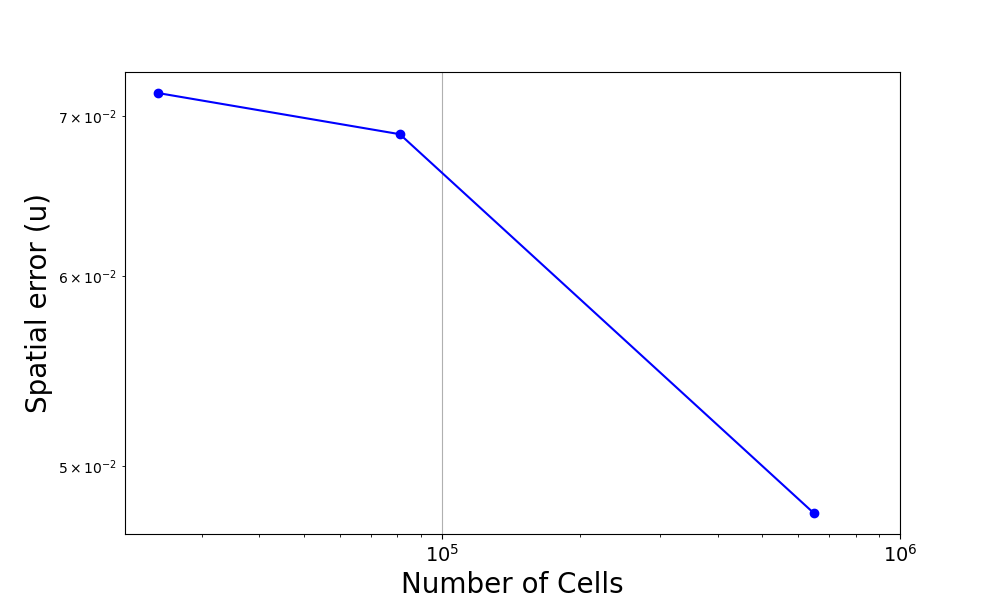
\includegraphics[width=16cm, height = 10cm]{ GWU_Thesis_Sarmakeeva/Images/chap3/l2_norm.png}
    \caption{$L2$ norm of the veolcity error obtained for the problem of a 3D falling sphere with CFDEMcoupling, for implemented solver with introduced a coupling force model.}
    \label{fig:l2}
\end{figure}

\begin{figure}[!ht]
    \centering
    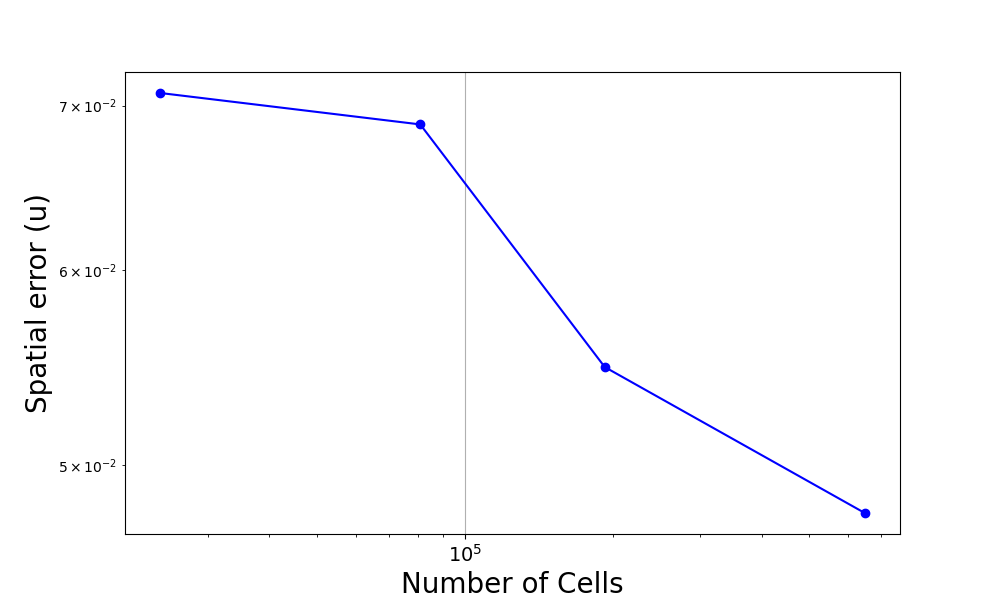
\includegraphics[width=16cm, height = 10cm]{ GWU_Thesis_Sarmakeeva/Images/chap3/l_inf.png }
    \caption{$L_{\infty}$ norm of the velocity error obtained for the problem of a 3D falling sphere with CFDEMcoupling, for implemented solver with introduced a coupling force model.}
    \label{fig:l_inf}
\end{figure}

The graphs provided on Fugure \ref{fig:l_inf}, and Fugure \ref{fig:l_2} represent the grid convergence study for a falling sphere simulation, showing how the average norm of velocity changes with the number of cells in the computational grid. 

The Fugure \ref{fig:l_inf} displays the $L_{\infty}$ norm of velocity error against the number of cells. The trend indicates that as the number of cells increases, the maximum velocity magnitude across the domain initially decreases sharply and then levels off, suggesting that a grid-independent solution is being approached. The plateau in the curve suggests that further refinement of the grid does not significantly change the maximum velocity, indicating that convergence has been reached for this norm.

The second graph Figure \ref{fig:l2} shows the $L2$ norm of velocity error against the number of cells. Similar to the $L_{\infty}$ norm results, the graph shows a decrease in the average $L2$ norm as the number of cells increases, with the rate of decrease diminishing as the number of cells becomes large. This suggests that the solution is approaching grid independence, where further refinement does not lead to significant changes in the overall velocity field as perceived by the $L2$ norm.


Implemented algorithm have different time communication between CFD and DEM solvers. Some-times to save computational resources it is common practice to set up communication every $5$ or $10$ computational steps, that mean that time-step would be for DEM part $10$ time smaller than for OpenFOAM solver.

To better understand how these parameters could affect the computations we completed analysis running for different setting for communication of coupled parts. Results provided on the Figure \ref{fig:communication} below.

\begin{figure}[!h]
    \centering
    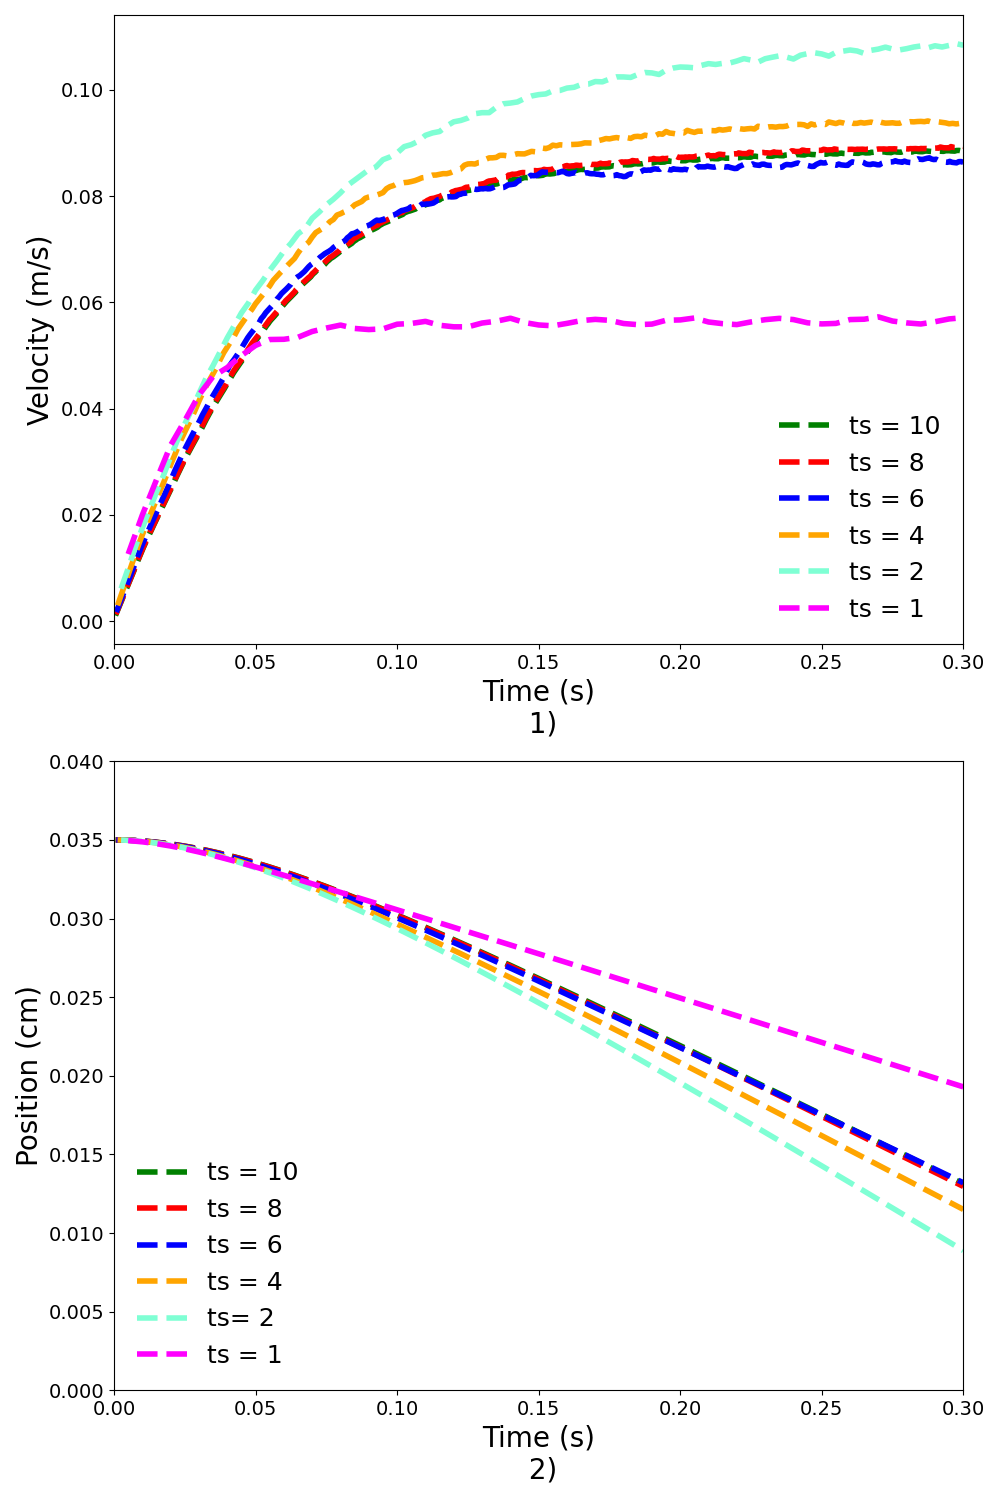
\includegraphics[width=13cm]{ GWU_Thesis_Sarmakeeva/Images/chap3/nan_simulation_192000_diff_exchange_time.png}
   \caption{Different setting for communication between CFD and DEM parts for every 10, 8, 6, 4, 2, 1 exchange time step  $ts$ 1) velocity component 2) change in z-direction.}
    \label{fig:communication}
\end{figure}

On the figure \ref{fig:communication} shown obtained data for the problem of a 3D falling sphere with CFDEMcoupling. It is implemented solver for the coupling force model, where $ts$ is the time step for data exchange. CFD and DEM solvers are communicating every 10th, 8th, 6th, 4th, 2nd, and each computational step correspondingly. The Figure \ref{fig:communication} shows that different exchange steps affect sphere's velocity and position, highlighting the critical role of exchange time step frequency in the numerical stability of the coupled scheme. Notably, a discrepancy in velocity is observed when comparing exchange steps $1$ and $2$. 

Further insights from a grid convergence study reveal an improvement in scheme stability with an increased cell count, underscoring the importance of grid refinement in simulation accuracy. The findings suggest that careful consideration of the exchange time step frequency and grid resolution is important for optimizing solver performance and ensuring the reliability of the simulation results.
\begin{figure}[H]
    \centering
    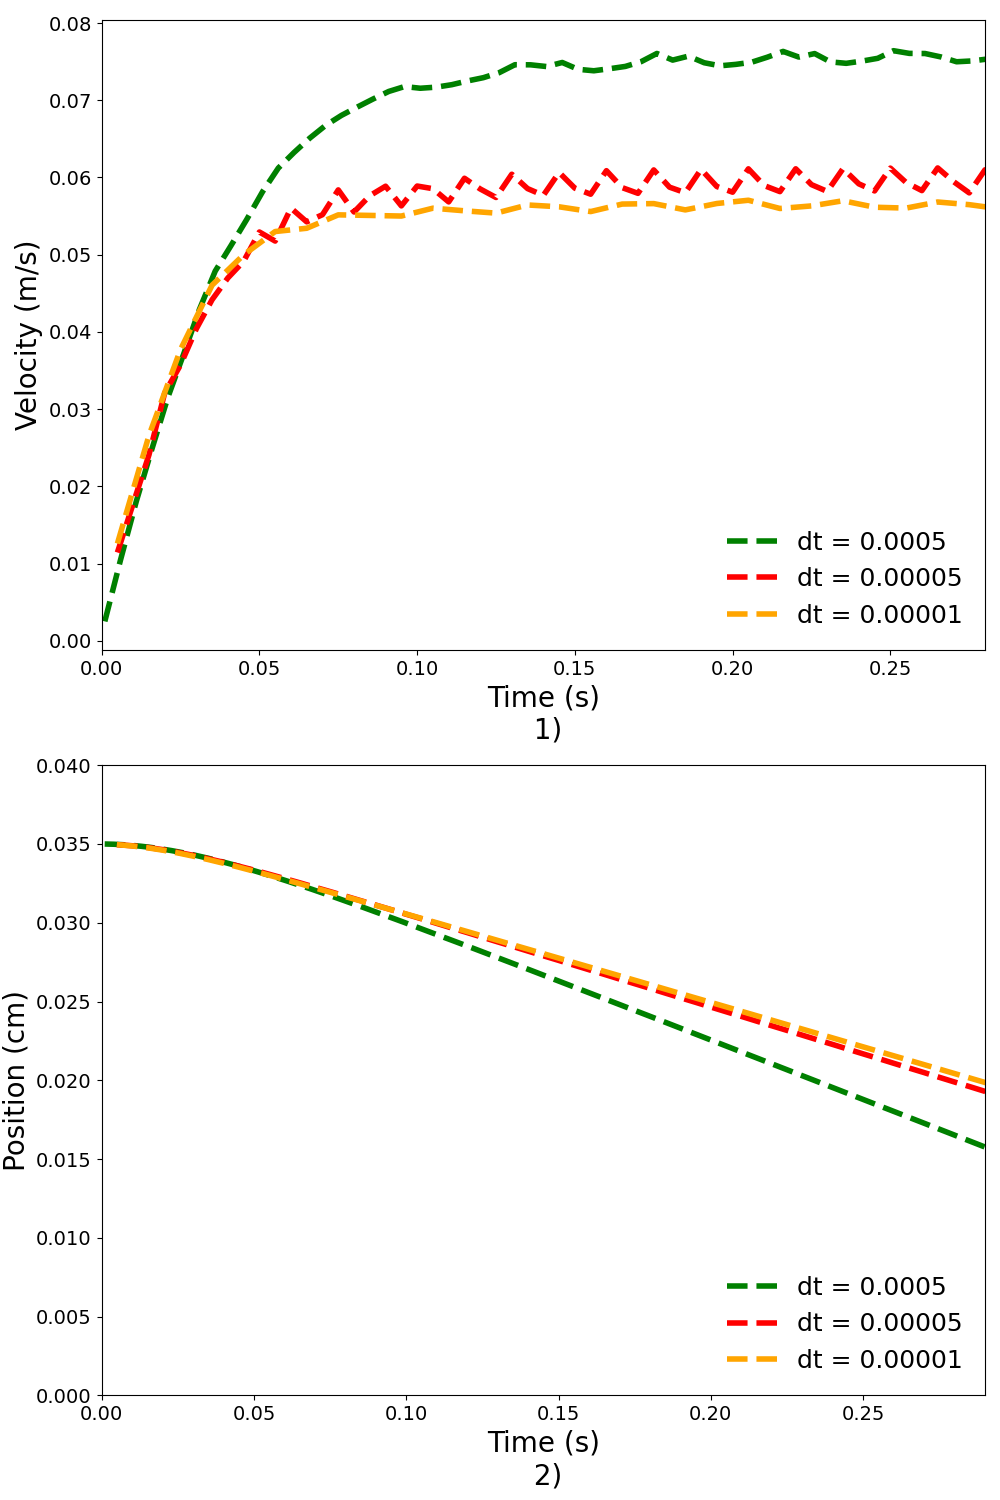
\includegraphics[width=12cm]{ GWU_Thesis_Sarmakeeva/Images/chap3/nan_simulation_192000_cells_dt_different.png }
    \caption{ Different setting for $\Delta t$ 1) velocity component 2) change in z-direction.}
    \label{fig:diff_dt}
\end{figure}

Another simulation was done, were computations of 3D falling sphere for the different time step. Results for $\Delta t = 0.00001$, $0.00005$ and $0.0001$ provided on the Figure \ref{fig:diff_dt}. For this experiment we used mesh for 192000 computational cells.
\begin{figure}[H]
    \centering
    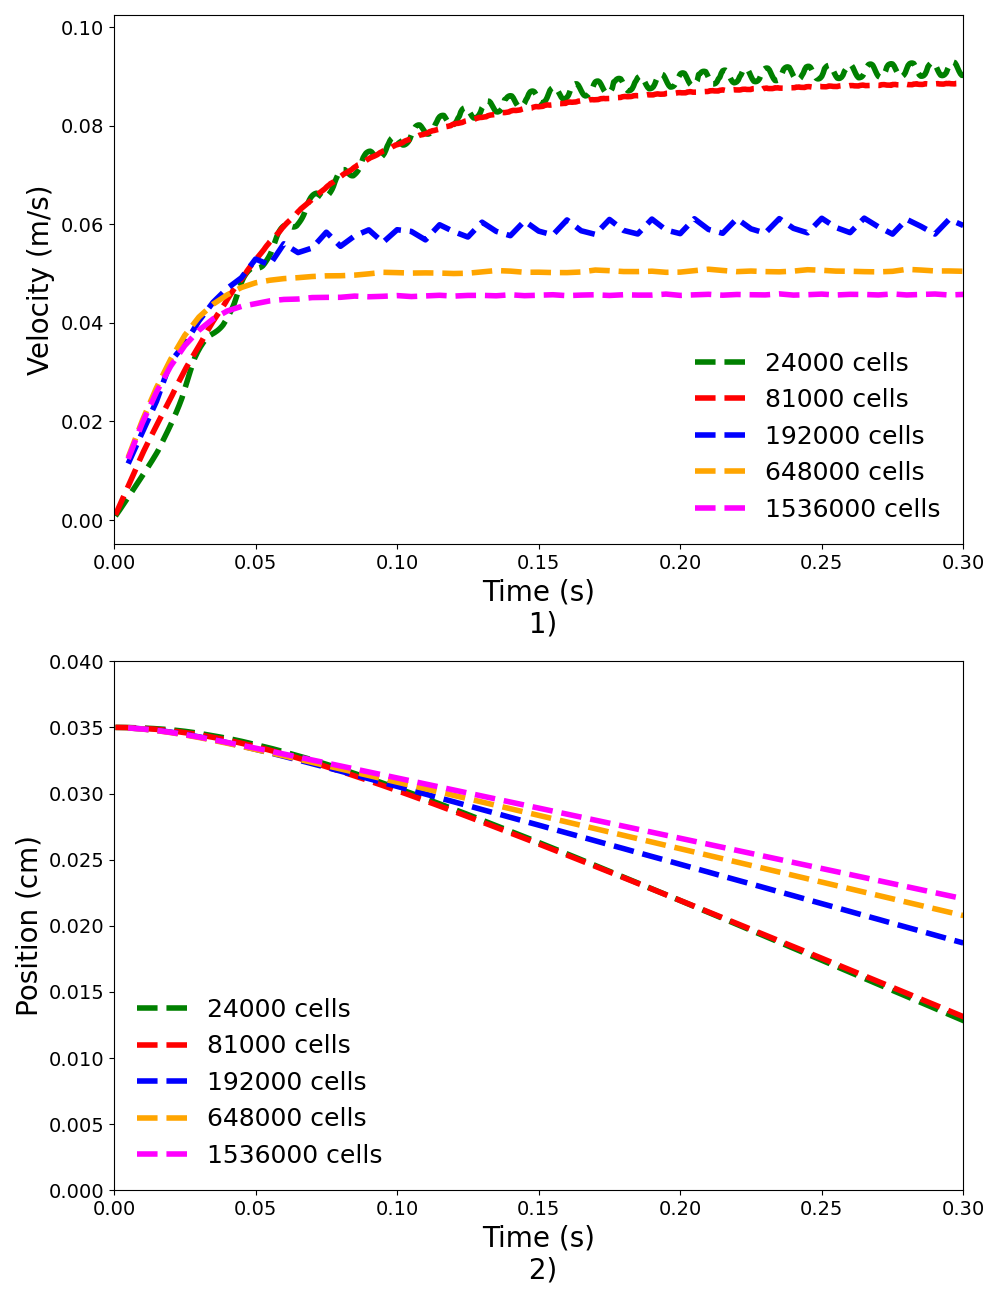
\includegraphics[width=14cm]{ GWU_Thesis_Sarmakeeva/Images/chap3/nan_simulation_192000_diff_cells_number.png}
    \caption{ Different setting for $\Delta x$: 1) velocity component 2) change in z-direction.}
    \label{fig:cell_num}
\end{figure}
As we can see from the results for the velocity change $\Delta t = 0.00005$ is unstable, but for $\Delta t = 0.00001$, and $0.0001$ they are stable showing significant error. Then we run experiments for different number of computational cells.

To calculate spatial error we run simulation consistently for different number of computational cells, parameters of the meshes provided in Table \ref{table1-chap4}:

\begin{table}[H]
    \centering
    \caption{Mesh Parameters for calculation spatial error. } \label{table1-chap4}
    \begin{tabular}{llll}
        \toprule
        \hline
        Name     & Cell number & dimensions&$x\times y \times z $\\
        \hline
        \midrule
        Mesh 1   & 24000 && 20 20 60\\
        Mesh 2 & 81000 & &30 30 90\\
        Mesh 3 & 192000 &&40 40 120 \\
        Mesh 4 & 648000 & &60 60 180 \\
        Mesh 5 & 1536000 & &80 80 240\\
        \hline
        \bottomrule
     \end{tabular}
\end{table}

In Figure \ref{fig:cell_num}, we observe distinct behaviors in the simulation results that correlate with the number of computational cells used in the mesh. The results of the coarser meshes with 24000 and 192000 cells exhibit instability, as evidenced by the divergence in the velocity and position curves. Conversely, the mesh with 81,000 cells yields more stable outcomes, yet there remains a notable deviation from the results obtained with higher-resolution meshes, indicating potential inaccuracies. This difference could be a consequence of the mapping algorithm used for calculations.

As the mesh is refined to 648,000 and 1,536,000 cells, the simulation results demonstrate improved stability and a trend toward convergence. The close agreement between these two higher-resolution meshes suggests that the solution is approaching a mesh-independent state, which indicates numerical convergence. This behavior implies that the discrepancies observed in coarser meshes may result from the mesh resolution and its interaction with the mapping algorithm. 


\section{The two phase experiments.}

In a subsequent validation phase, we extended the simulation to include a multi-spherical body designed to mimic the shape and dimensions of the single falling sphere. This experiment assessed the solver's capability to approximate complex particle shapes while maintaining the same fluid and particle parameters outlined in Table \ref{table1-chap4}.

\begin{table}[H]
    \centering
    \caption{Simulation Parameters} \label{table2-chap4}
    \begin{tabular}{llr}
        \toprule
        \hline
        Simulation Part         & Physical Parameters (units) & Value \\
        \hline
        \midrule
        Particle                 & Density (kg/m$^3$)          & 500    \\
                         & Diameter (cm)          & $0.252$    \\
                         & Initial height (cm)          & $1.0252$    \\
                         \hline
        Fluid                  & Density (kg/m$^3$)           & $1000$   \\
                                & Viscosity (m$^2$/s)         & 1e$^{-6}$    \\
                                \hline
         Air                  & Density (kg/m$^3$)           & $1e-5$   \\
                                & Viscosity (m$^2$/s)         & 1e$^{-6}$    \\
                                \hline
        \bottomrule
     \end{tabular}
\end{table}
Figures \ref{fig:two-phase_sphere} and \ref{fig:IB} present the simulation outcomes for the multi-spherical body from the published work and our solver, respectively. Results shows good agreement. For a more quantitative insight, Figure \ref{fig:2ph_exp} displays the trajectory in the $z$-direction of the falling sphere.

\subsection{A bouncing sphere example, water-air}
The initial experiment comes from the work \cite{beck1987transient}. Where they using the tank parameters: length: 109.7 m, width 6.7 m, depth 3.2 m. The sphere radius $r= 0.254$ m , height $z = r/10$ above the free surface. The sphere density 500 kg/m .

First, we tried to make regular mesh similar to Pathak etc.\cite{pathak20163d} work. For the domain size from Pathak etc.\cite{pathak20163d} we followed formula:
\begin{equation}
    (length \cdot height \cdot width)  \cdot  r  \cdot  CPR,
\end{equation}
where CPR - cell per radius of sphere. To safe computational resources for tank $13\times 6.7 \times 3.4$ $\approx 17$ M cells with CPR $= 10$.
 $\approx 8$ M cells for tank $5\times 5 \times 5$, CPR $= 10$
 $\approx 2.7$ M cells for tank $5\times 5 \times 5$ with mesh refinement to the center, CPR $= 10$

For the lowest mesh resolution results of simulation shown on the figure below \ref{fig:2ph_exp}.
\begin{figure}[!ht]
    \centering
    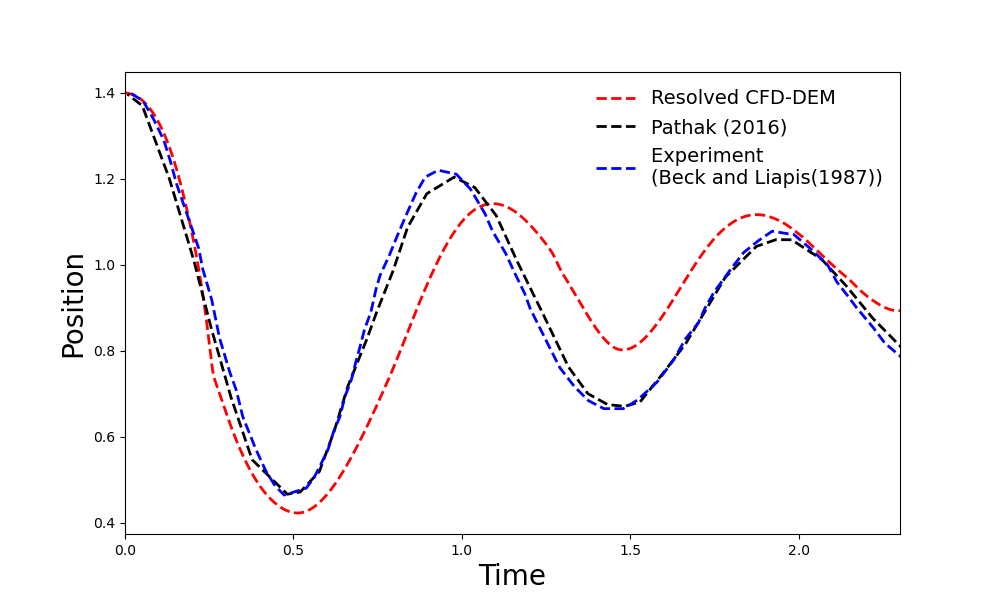
\includegraphics[width=15cm]{Images/chap3/bouncing_sphere_plot.png}
    \caption{Bouncing sphere simulation for two-phase fluid from the CFD-DEM simulation}
    \label{fig:2ph_exp}
    \end{figure}
The main parameters shown in the Table \ref{table2-chap4}. 

Figure \ref{fig:two-phase_sphere} provided a series of time-step snapshots from a CFD-DEM simulation of a sphere interacting with a two-phase fluid, where dark blue is a liquid with the density of water and light blue is a liquid with the density of the air.

\begin{figure}[H]
    \centering
    \begin{minipage}{.4\textwidth}
        \centering
        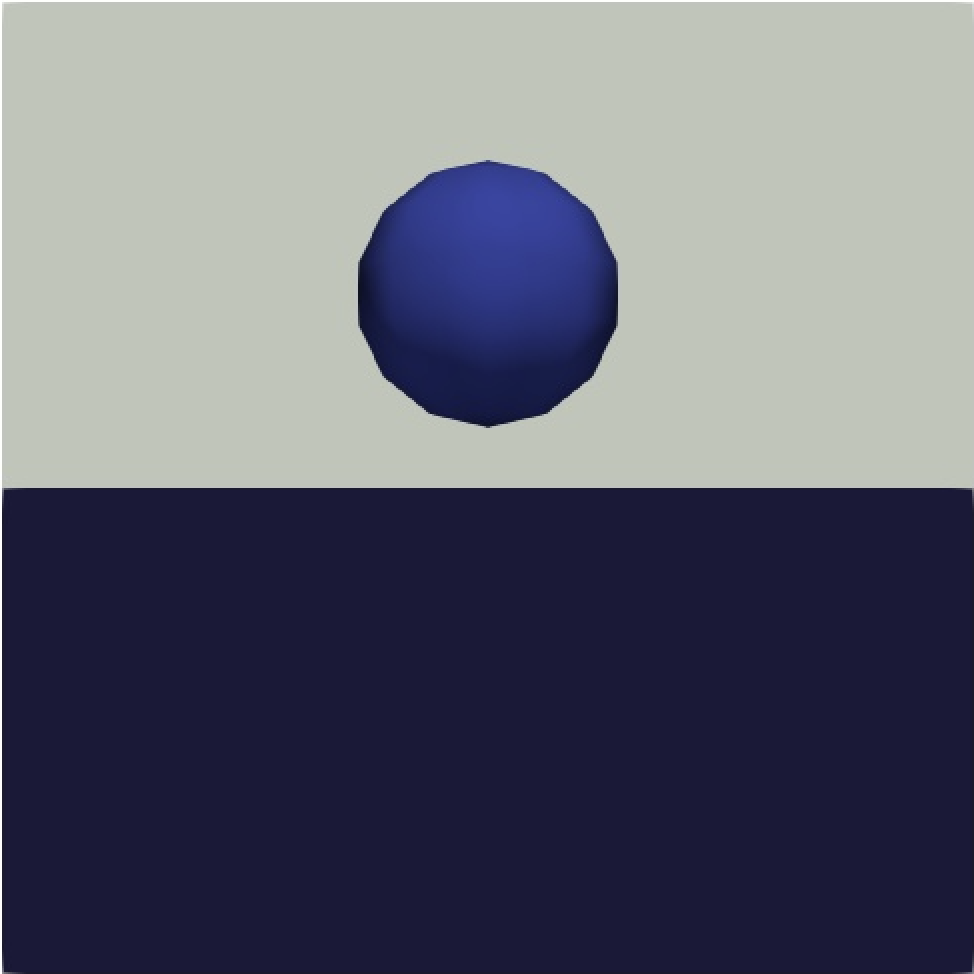
\includegraphics[width=\linewidth]{GWU_Thesis_Sarmakeeva/Images/chap4/water_sphere/sphere_in_water0.png}
        \subcaption{0.1 sec}
    \end{minipage}%
    \hspace{0.05\textwidth}
    \begin{minipage}{.4\textwidth}
        \centering
        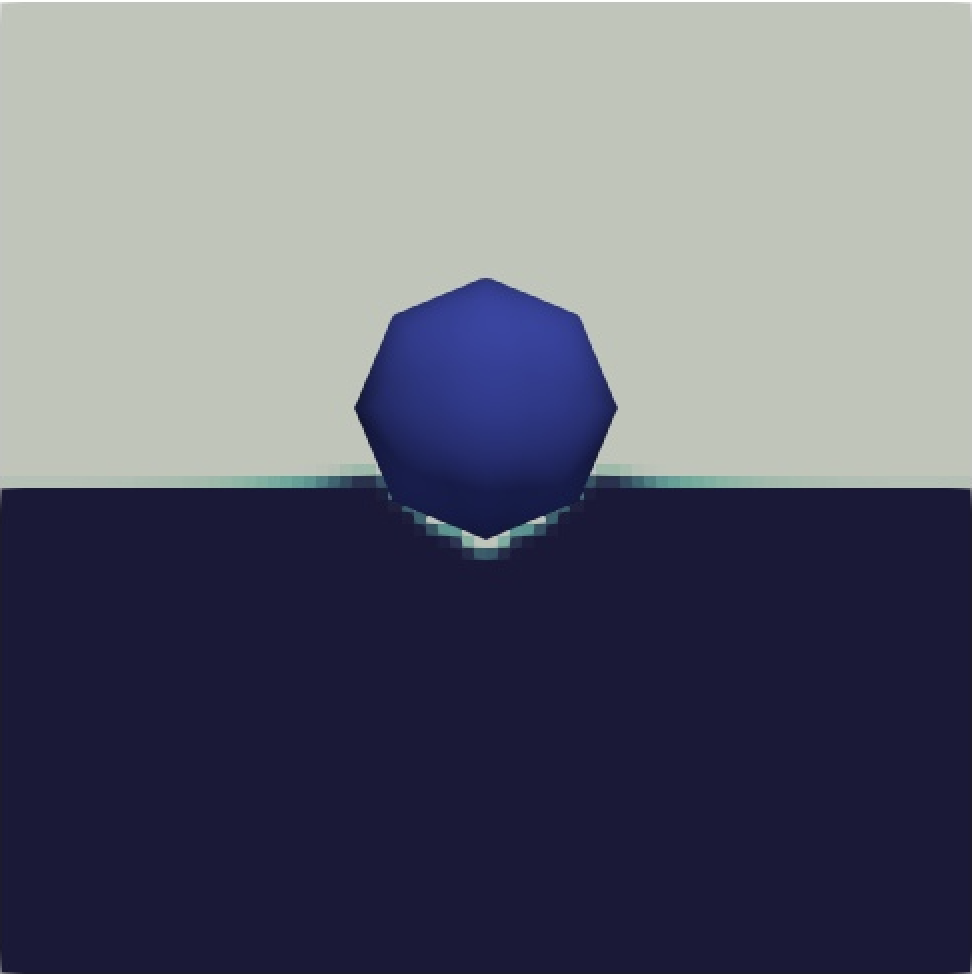
\includegraphics[width=\linewidth]{GWU_Thesis_Sarmakeeva/Images/chap4/water_sphere/sphere_in_water02.png}
        \subcaption{0.2 sec}
    \end{minipage}
    \newline
    \begin{minipage}{.4\textwidth}
        \centering
        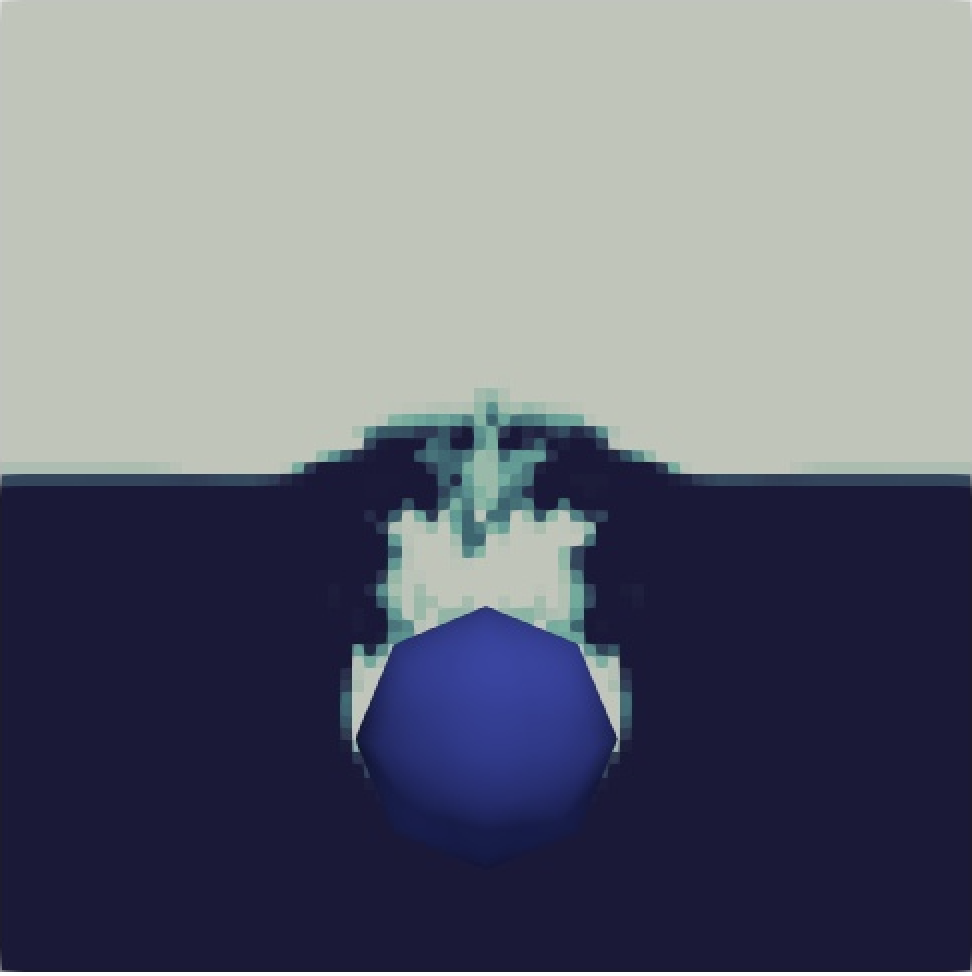
\includegraphics[width=\linewidth]{GWU_Thesis_Sarmakeeva/Images/chap4/water_sphere/sphere_in_water04.png}
        \subcaption{0.4 sec}
    \end{minipage}%
    \hspace{0.05\textwidth}
    \begin{minipage}{.4\textwidth}
        \centering
        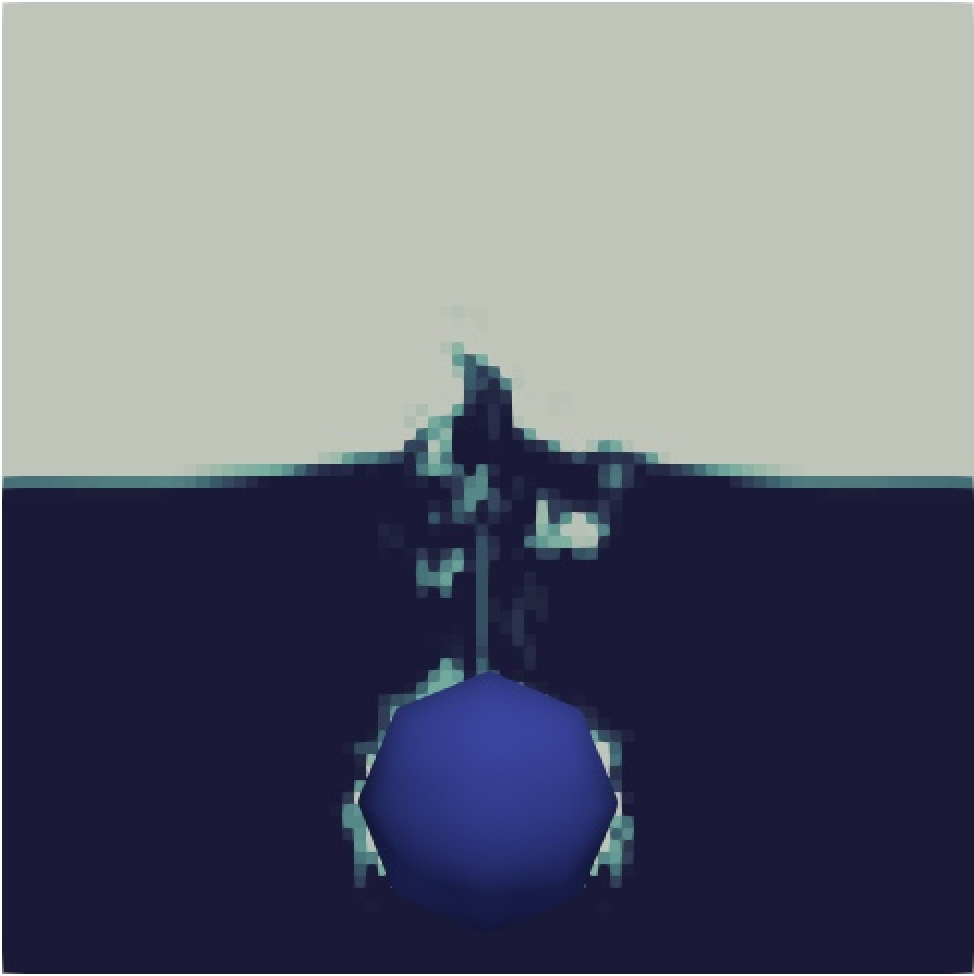
\includegraphics[width=\linewidth]{GWU_Thesis_Sarmakeeva/Images/chap4/water_sphere/sphere_in_water07.png}
        \subcaption{0.7 sec}
    \end{minipage}
    \newline
    \begin{minipage}{.4\textwidth}
        \centering
        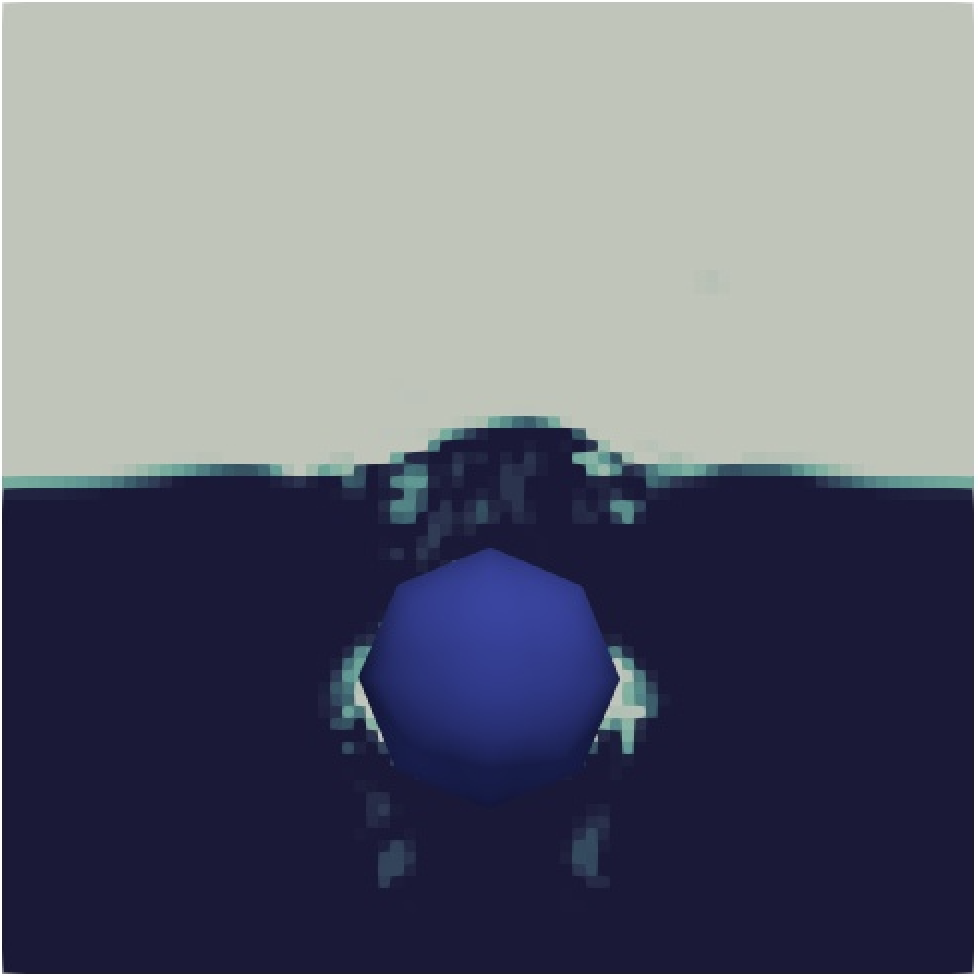
\includegraphics[width=\linewidth]{GWU_Thesis_Sarmakeeva/Images/chap4/water_sphere/sphere_in_water09.png}
        \subcaption{0.9 sec}
    \end{minipage}%
    \hspace{0.06\textwidth}
    \begin{minipage}{.4\textwidth}
        \centering
        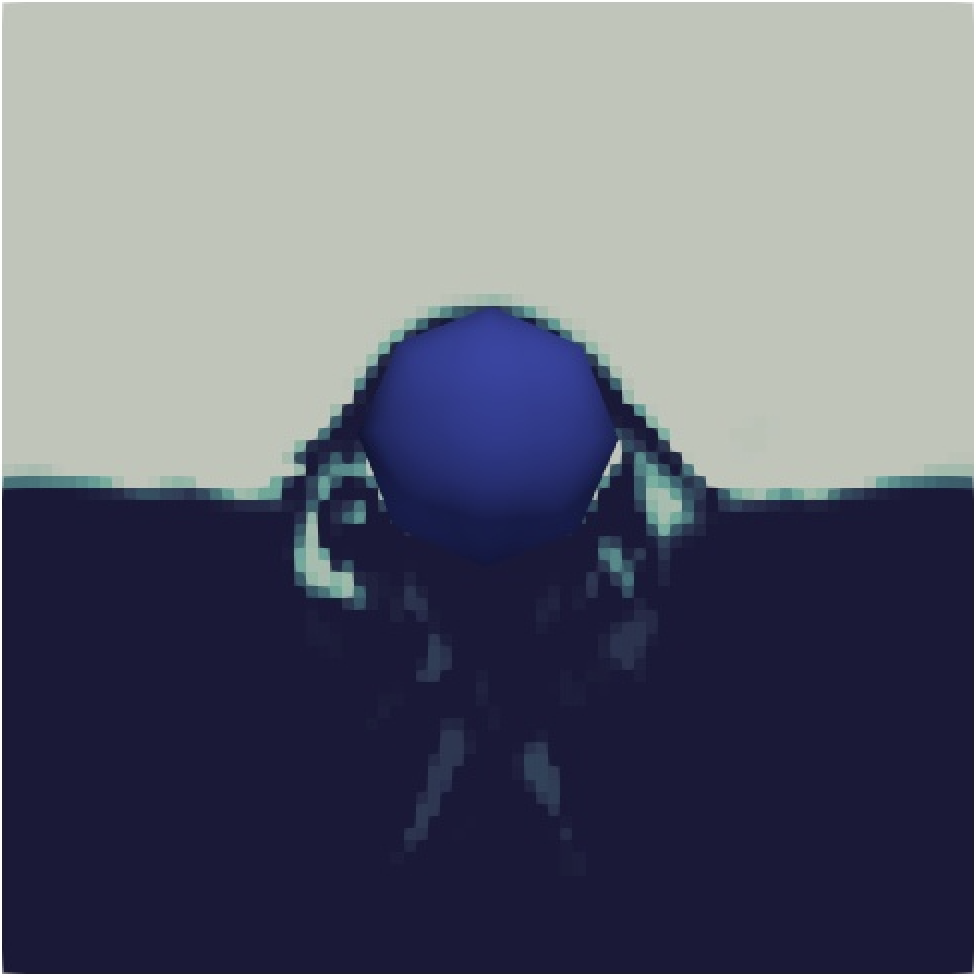
\includegraphics[width=\linewidth]{GWU_Thesis_Sarmakeeva/Images/chap4/water_sphere/sphere_in_water12.png}
        \subcaption{1.2 sec}
    \end{minipage}
    \caption{Visualization of sphere bouncing in two-phase fluid from CFD-DEM simulation.}
    \label{fig:two-phase_sphere}
\end{figure}
\begin{itemize}
    \item \textbf{Initial Contact (a - 0.1 sec):} The sphere is shown just above the fluid interface, moving under gravity force in the direction of the water
    \item \textbf{Entry and Deformation (b - 0.2 sec):}As the sphere impacts the fluid surface, we see the beginning of deformation at the fluid interface, indicating the sphere's entry into the water. The fluid is distorted in response to the sphere's presence, which illustrates the initial splash or the beginning of the sphere's submersion.
    \item \textbf{Submersion and Displacement (c - 0.4 sec):}The sphere is now submerged, and we can observe the water deforming significantly around the sphere, likely due to the displacement of water as the sphere moves downward. Which shows numerical stability
    \item \textbf{Maximum Penetration (d - 0.7 sec):}This image might represent the sphere at or near its maximum depth, given the substantial fluid displacement.
    \item \textbf{Upward Motion (e - 0.9 sec):}The sphere is moving upward, indicating that it is buoyant as indicated by the changing flow patterns and the 'tail' of disturbed fluid below it.
    \item \textbf{Surface Re-contact (f - 1.2 sec):}The sphere has ascended back to the fluid interface, and we can see the water's surface tension is deformed as the sphere pushes up against it, about to break through the surface again
\end{itemize}

This simulation is essential to test the numerical stability of the algorithm for surface tension calculation of the numerical scheme, and experiments confirm it.

 \begin{figure}[!ht]
    \centering
    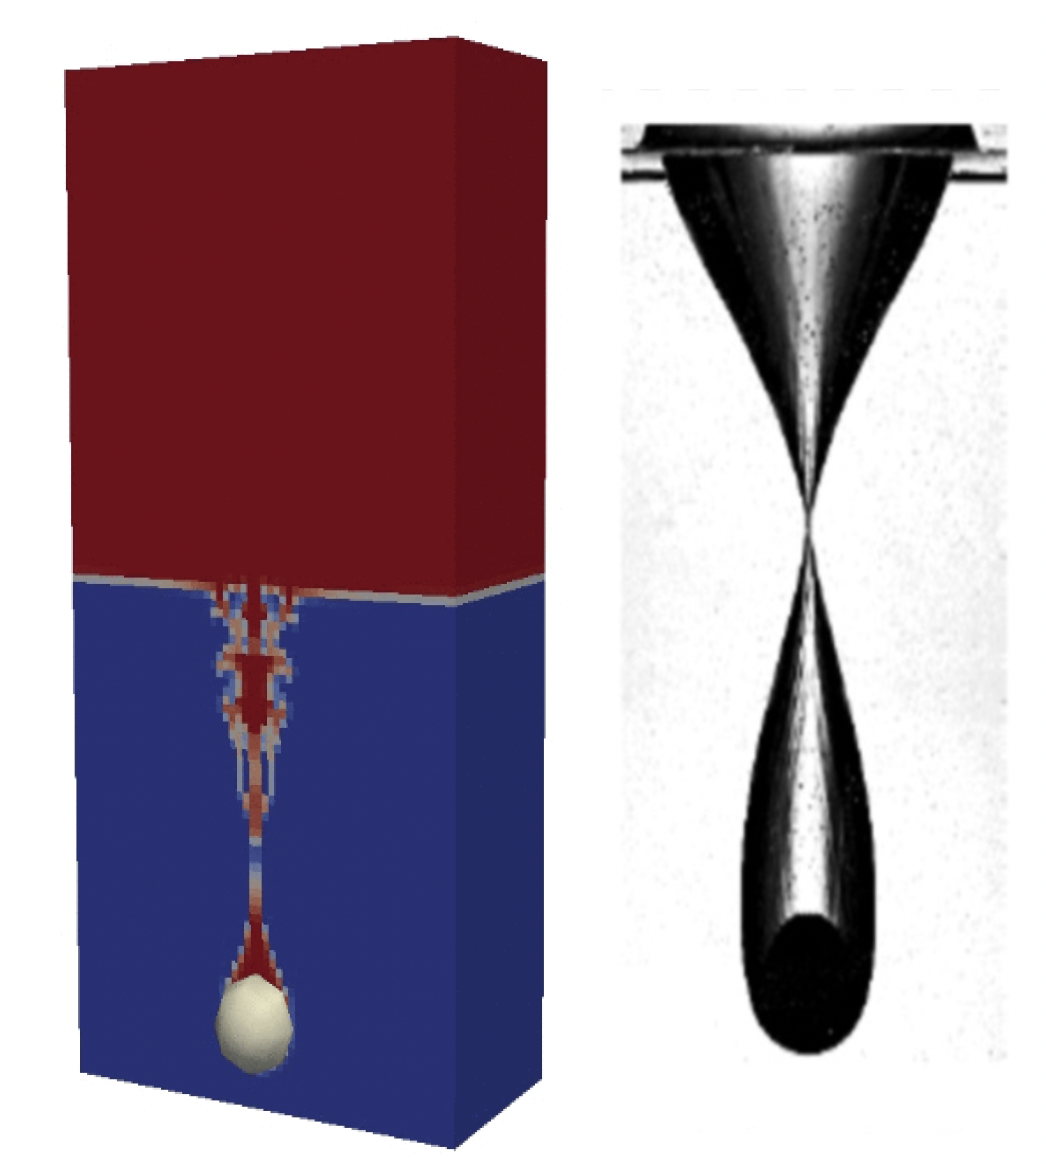
\includegraphics[width=12cm]{Images/chap3/cavityIB.png}
    \caption{Falling sphere visualization results. On the right, cavity after falling sphere in the water \cite{schwalbach}.}
    \label{fig:IB}
\end{figure}
Reproducing the physical experiments involving a sphere falling into the water where density of the sphere more than water, as outlined in \cite{schwalbach}, have challenges for numerical comparison. One primary obstacle is that the original paper needs to include the height from which the sphere is dropped. This parameter has a significant impact on the free surface during the simulation and is essential for ensuring the stability of our solver. Despite this, the trajectory of the falling sphere in our simulations aligns well with the physical experiments, suggesting that our results are both stable and comparable. Another study, \cite{shen2022resolved}, also attempts to replicate the original experiment through numerical methods. Again, this paper, in the same way, neglects to specify the height from which the spheres were dropped, making a complete comparison of results problematic.

\subsubsection{Computational setup}

For the numerical simulation we choose IsoAdvector \cite{roenby2019isoadvector} method for simulation of free surface which is described in a theoretical part. Applying second order Crank–Nicolson method for time differentiation . For interpolation  diffusion and convection terms we used scheme which called \textit{Gauss linear} in OpenFOAM, which is the second-order accurate scheme, the standard finite volume discretization using the Gaussian integration that requires the interpolation from cell centers to face centers. Pressure field tolerance was chosen as $1e-06$. With 3 PISO loops on each time step. The time step we choose $\Delta t = 1e-05$ for the VOF part and $\Delta t = 1e-06$ for the DEM part i.e communication was made every $10$ time steps from the solid body part.

We carried out the simulations of a high-performance computing system. The key specifications of the system CPU: AMD Ryzen Threadripper PRO 3995WX, 64-Core, 128-Thread, with frequencies ranging from 2200 MHz to 4308.4 MHz. System Architecture: x86\_64, supporting 32-bit and 64-bit operations. Operating System: Linux-based.
\section{Multispherical body simulations}

\subsection{Multispherical body interaction with two-phase fluid}

The primary objective of this experiment is to illustrate initial stability and functionality of the developed CFD-DEM code through simulating the interaction of a multi-spherical body, analogous to a previous experiment with a floating sphere in water.

The simulation involve es a multi-spherical body consists out of 2 overlapping spheres, positioned at a $0.4$ m height above a fluid with the proprieties of water. The main properties are provided in the Table \ref{table3-chap4} below.
\begin{table}[H]
    \centering
    \caption{Simulation Parameters} \label{table3-chap4}
    \begin{tabular}{llr}
        \toprule
        \hline
        Simulation Part         & Physical Parameters (units) & Value \\
        \hline
        \midrule
        Particle 1                & Density (kg/m$^3$)          & 500    \\
                         & Diameter (m)          & 0.25    \\
                         & Initial height (m)          & (0.5, 0.5, 1.4 )  \\
        Particle 2                & Density (kg/m$^3$)          & 500    \\
                         & Diameter (m)          & 0.25   \\
                         & Initial height (m)          &  (0.2, 0.4, 1.4)     \\
                         \hline
                                 Fluid                  & Density (kg/m$^3$)           & $1000$   \\
                                & Viscosity (m$^2$/s)         & 1e$^{-6}$    \\
                                \hline
         Air                  & Density (kg/m$^3$)           & $1e-5$   \\
                                & Viscosity (m$^2$/s)         & 1e$^{-6}$    \\
                                \hline
        \bottomrule
     \end{tabular}
\end{table}

The body is released and allowed to fall into the water under gravity forces. The simulation captures the motion of the body and the fluid's response upon impact and during the subsequent settling period. The results of simulation showed on a figure \ref{fig:two-phase exp} below.

\begin{figure}[!ht]
  \centering
  \begin{tabular}{cc}
    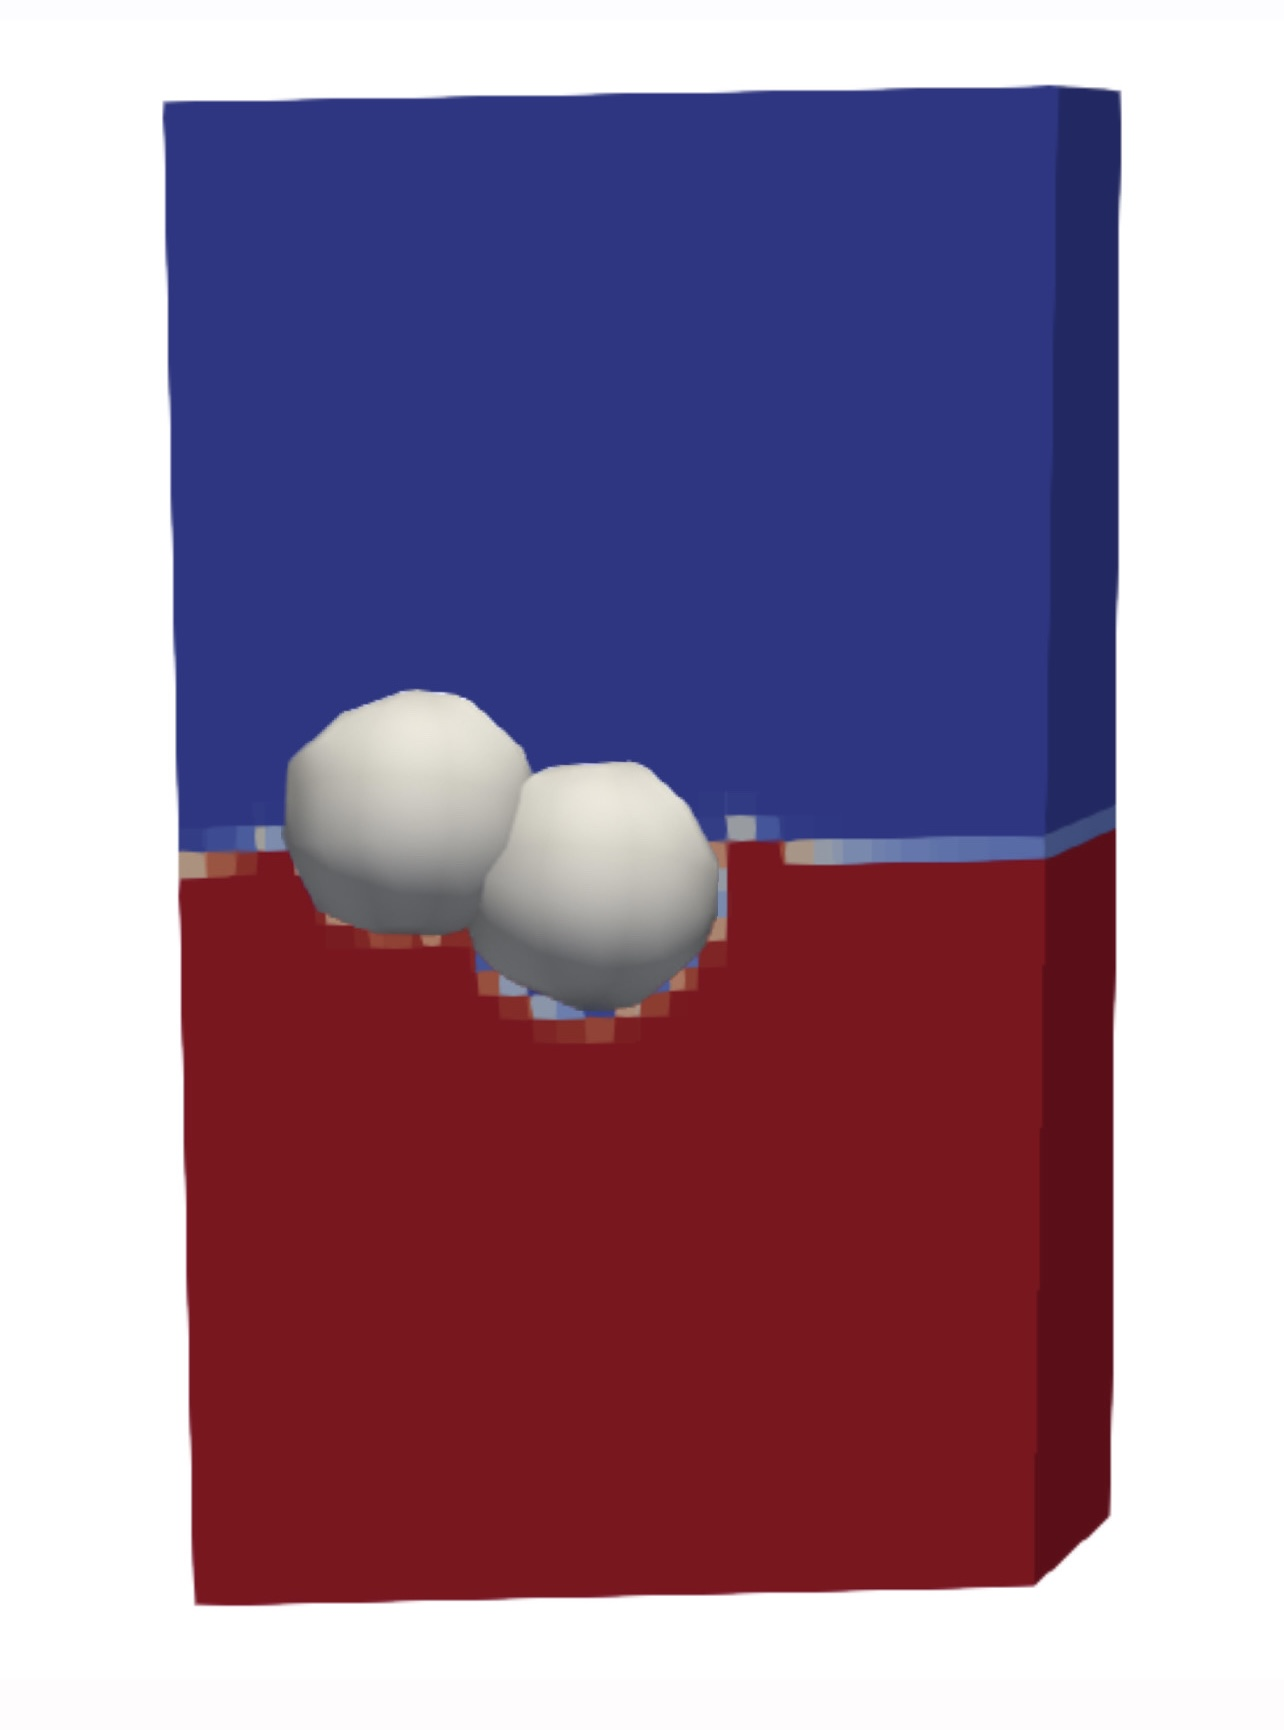
\includegraphics[width=0.4\textwidth]{Images/chap3/2_sph_2.jpg} & 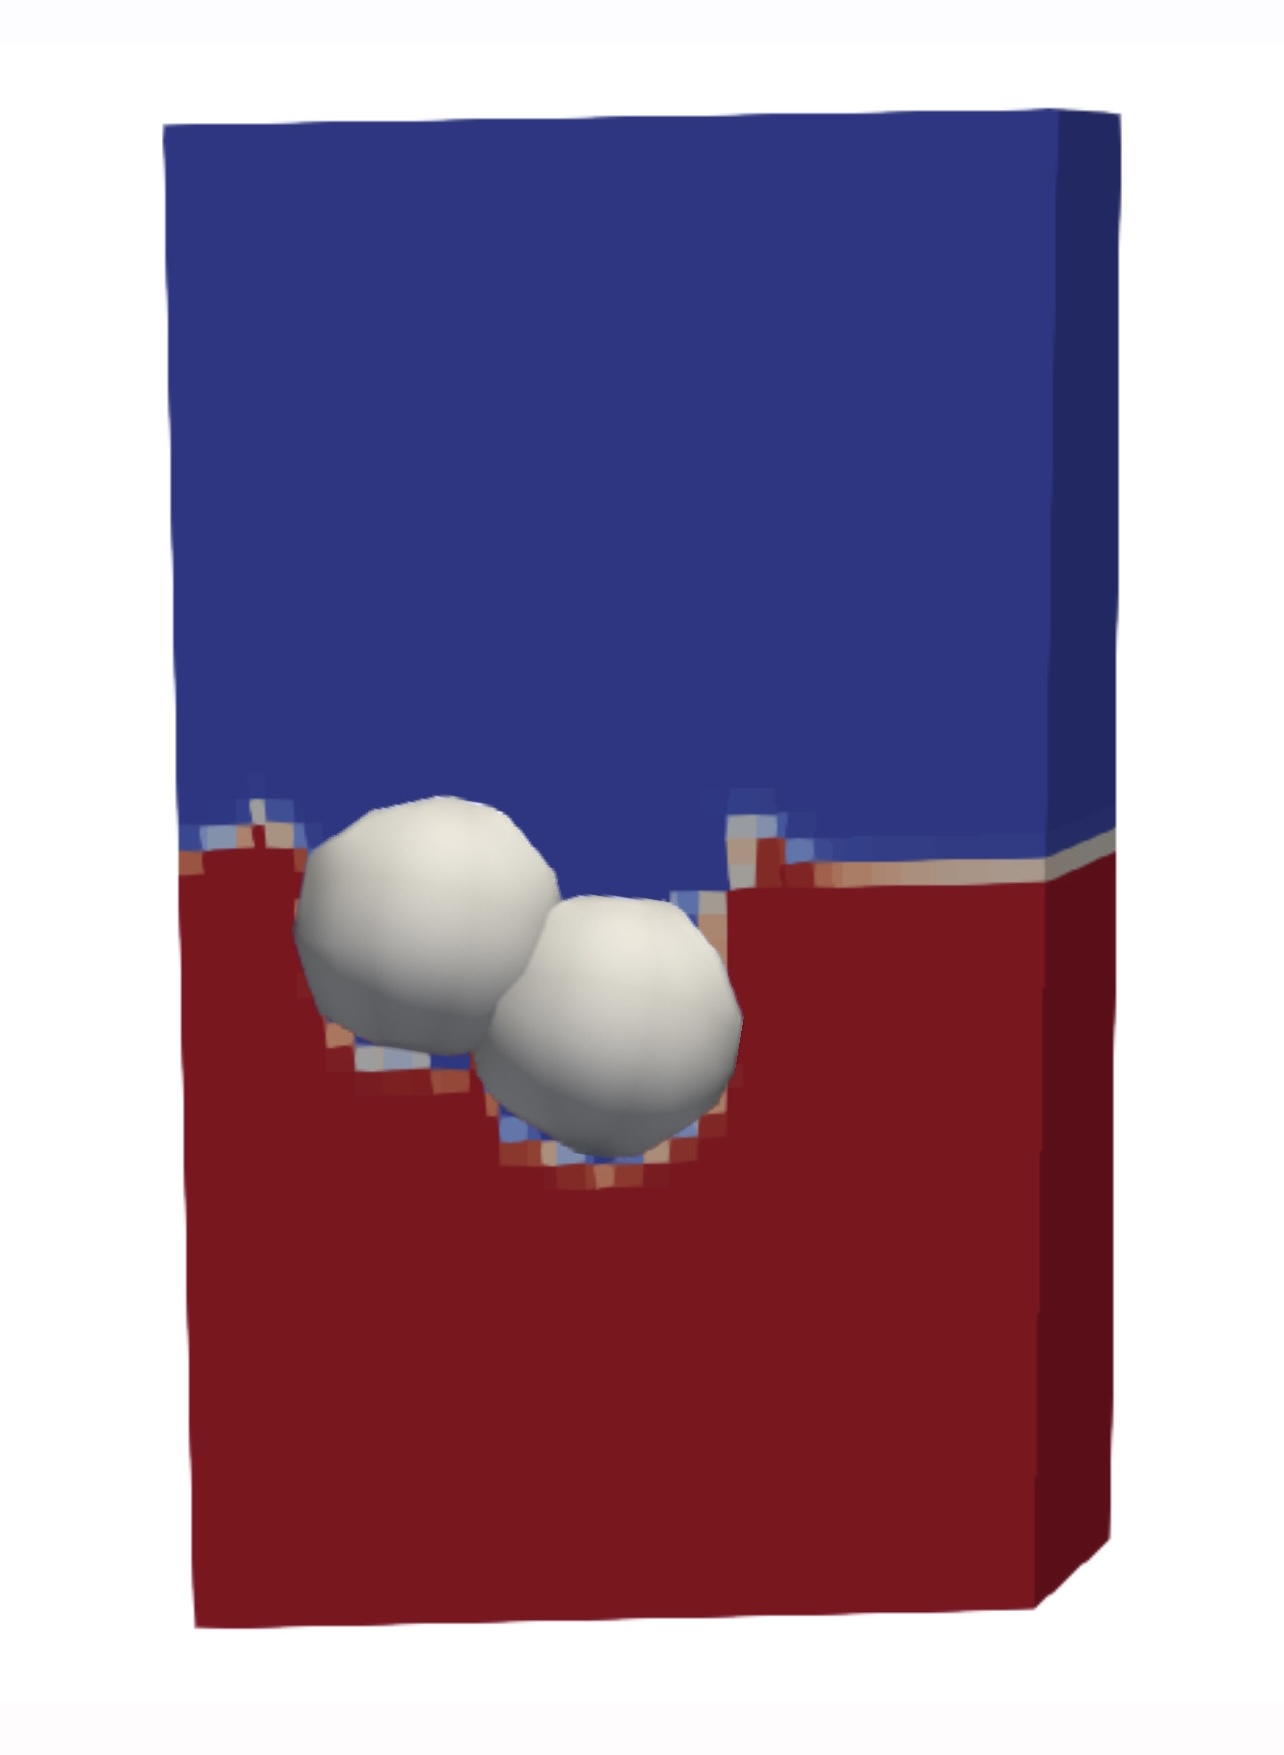
\includegraphics[width=0.4\textwidth]{Images/chap3/2_sph_1.jpg} 
    %(a) 0. s & (b) 0.35 s \\
  \end{tabular}
  \caption{Multispherical body created out of two spheres bouncing in liquid.}
  \label{fig:two-phase exp}
\end{figure}

The results of simulation showed numerical stability of the solver. Another concern was the volume of fluid phases, it changes in the range less than 1\%.

\subsection{Multispherical sinking body simulations}

A couple of works use similar approaches recently published for landslide simulations as \cite{nan2023high} and \cite{shen2022resolved}.
Like them, we run the simulations with one multi-spherical body falling into the water and multiple arbitrarily shaped bodies falling under gravity force, interacting with each other and interacting with water.

First, we would consider the falling clump - multispherical body experiment \ref{fig:two-phase_exp}. The solid body is made out of $50$ intersecting spheres with the density of 2500 kg/m$^3$ and set up in the area $x: 0.15 $ to $0.22$, $y: 0.1$ to $0.125$, $z: 0.3$ to $0.35$. CFD domain is $0.4\times 0.3\times0.4$. The fluid level is on $y = 0.2$. Simulation run for $0.3$s with $\Delta t = 5e-5$. The body falling under gravity force in $z$-direction. 

The image \ref{fig:two-phase_exp} captures the dynamic interaction between the multispherical body and the fluid, including the entry, sinking, and settling phases. The snapshots highlight the complexity of movement and deformation of a clump. Figure\ref{fig:two-phase exp}(a) shows the initial multispherical body placement, which is located between $0.3$ and $0.35$, the body starts to fall under the gravity force. In the second image \ref{fig:two-phase_exp} (b), we can see the body after penetration into the water. In figures \ref{fig:two-phase_exp} (c) and (d), we can see the body settled at the bottom of the container, and the fluid's free surface is stabilized.

The simulation result shows the stability of the numerical scheme for the resolved CFD-DEM method as well as during fluctuations of free surface and calculation of surface tension. Due to successful multispherical body interaction with fluid, for the next simulation, we increased the number of clumps but reduced the number of spheres in clumps. 

\begin{figure}[!ht]
    \centering
    \begin{minipage}{.5\textwidth}
        \centering
        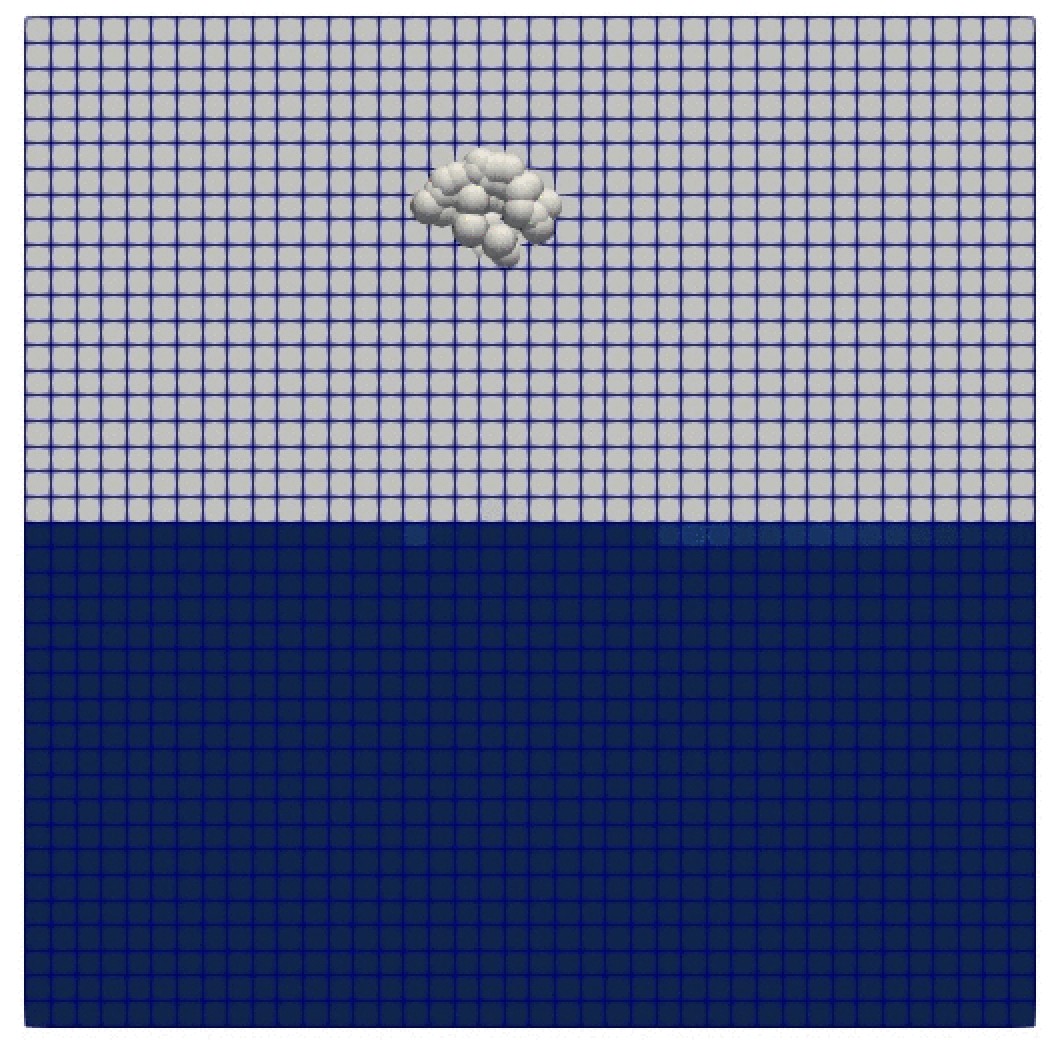
\includegraphics[width=\linewidth]{GWU_Thesis_Sarmakeeva/Images/chap4/clump_1.png}
        \subcaption{0 sec}
        %(a) 0. s
    \end{minipage}%
    \begin{minipage}{.5\textwidth}
        \centering
        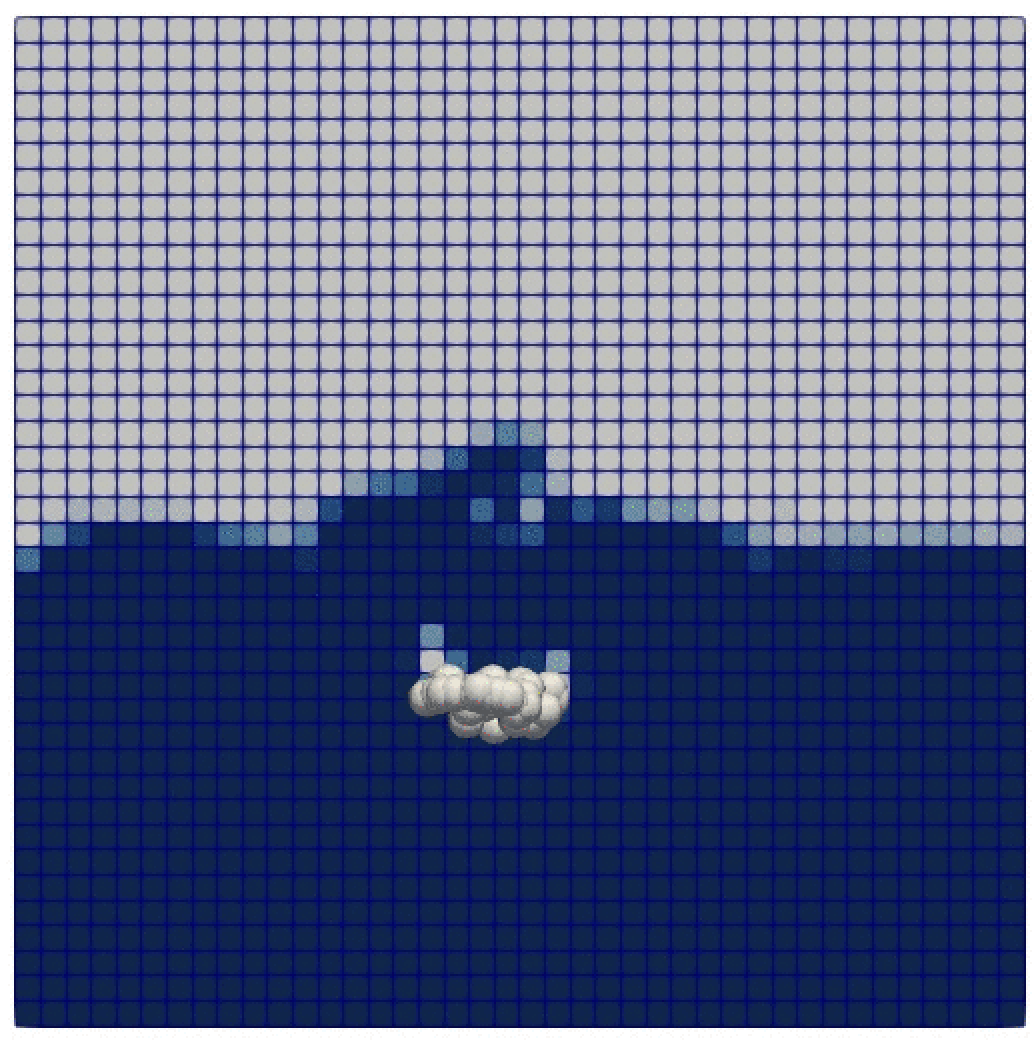
\includegraphics[width=\linewidth]{GWU_Thesis_Sarmakeeva/Images/chap4/clump_2.png}
        \subcaption{0.1 sec}
        %(b) 0.35 s
    \end{minipage}
    \newline
    \begin{minipage}{.5\textwidth}
        \centering
        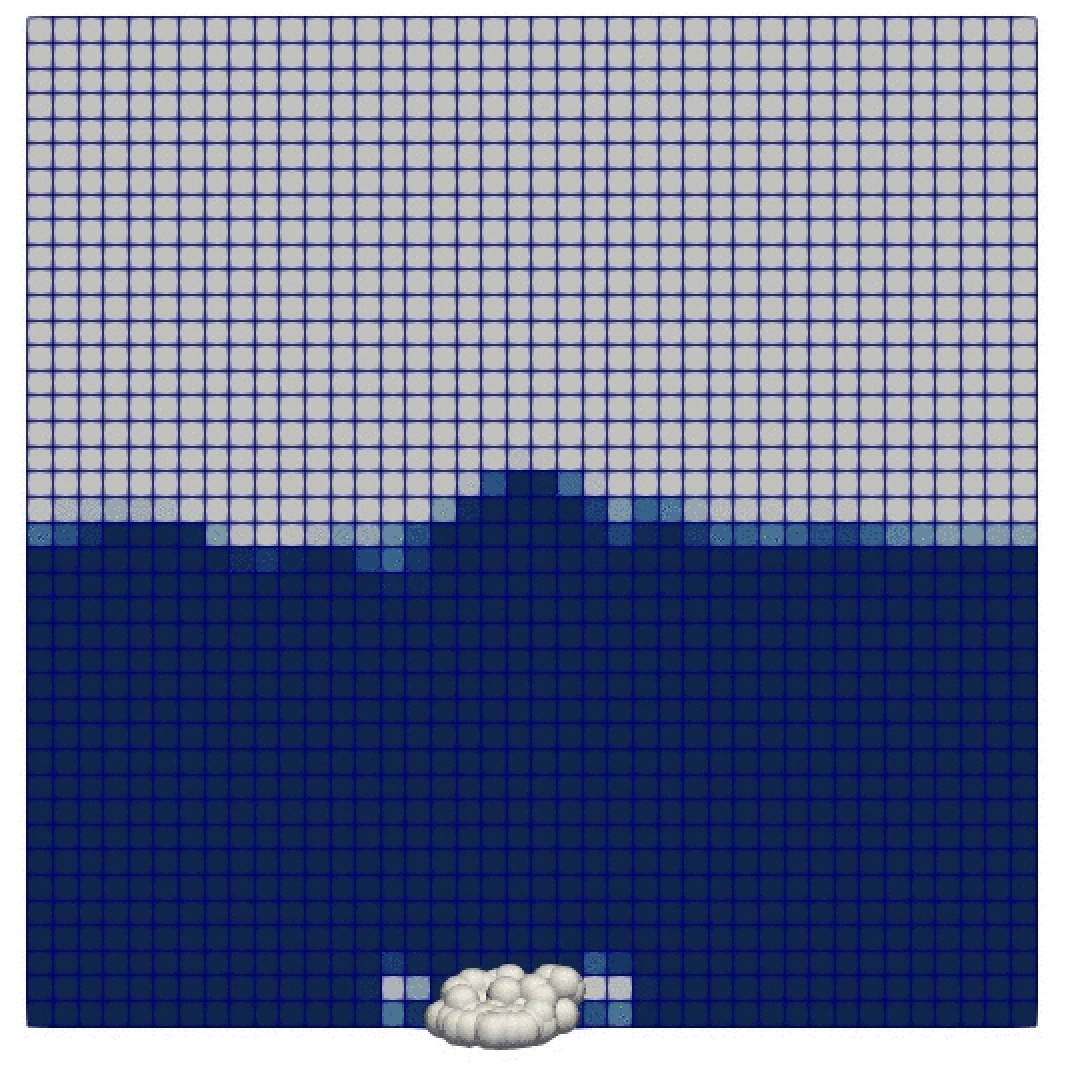
\includegraphics[width=\linewidth]{GWU_Thesis_Sarmakeeva/Images/chap4/clump_3.png}
        \subcaption{0.2 sec}
        %(c) Description
    \end{minipage}%
    \begin{minipage}{.5\textwidth}
        \centering
        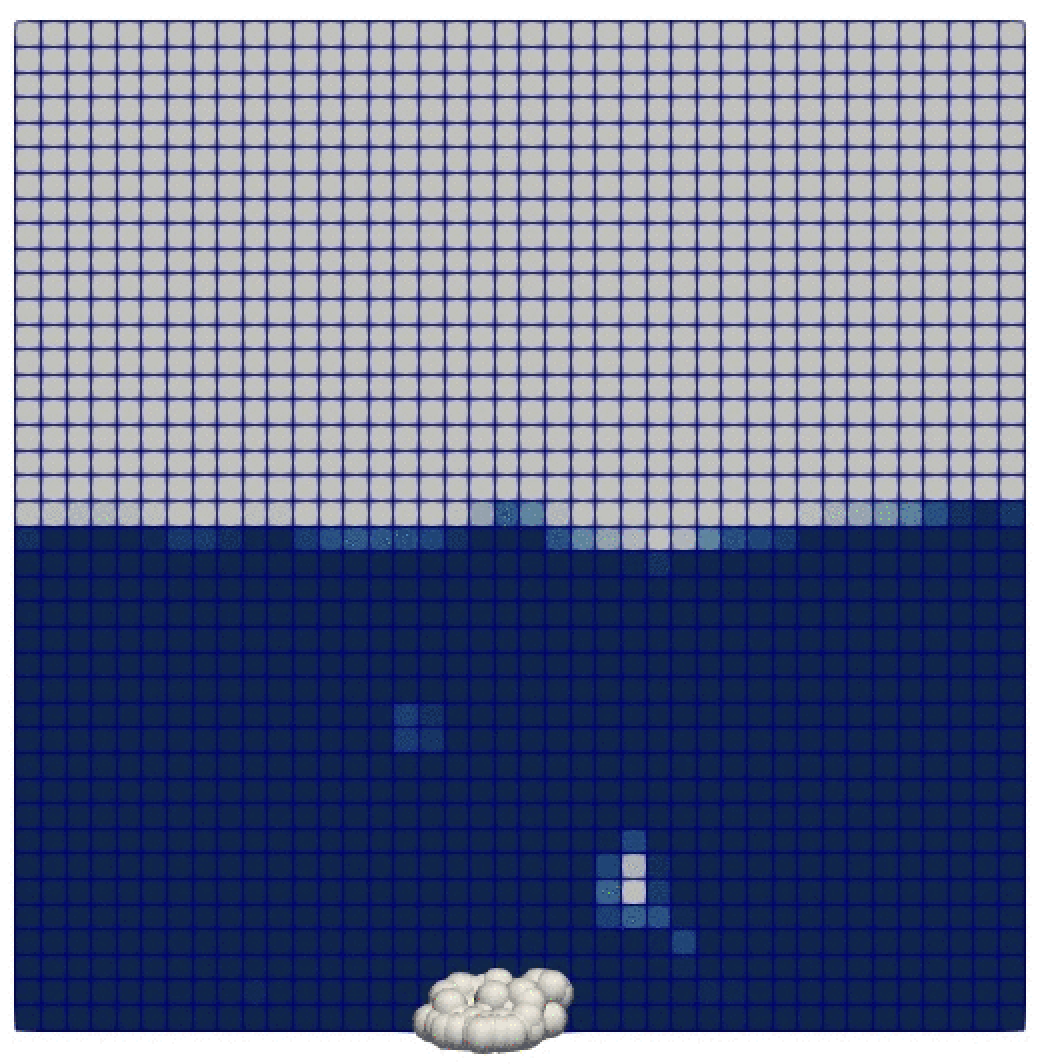
\includegraphics[width=\linewidth]{GWU_Thesis_Sarmakeeva/Images/chap4/clump_4.png}
        \subcaption{0.3 sec}
        %(d) Description
    \end{minipage}
    \caption{Falling multispherical body consisting of $n = 50$ spheres where a) initial clump placement b) after penetration into fluid c) body settled at the bottom of the container at 0.2 sec d) body settled at the bottom of the container at 0.3 sec}
    \label{fig:two-phase_exp}
\end{figure}

For multiple clumps simulation (Figure \ref{fig:two-phase_exp_clumps}), the experiment includes 22 clumps made out of 18 spheres, in total 396 spheres falling under gravity force and interacting with the splashed water. CFD area has 216000 computational cells, and the dimension of the domain is $0.4\times 0.3\times0.4$. Area filled with clumps is $x:0.2$ to $0.4$, $y: 0.0$ to $ 0.2$,$ z:0.0$ to $ 0.3$.
\begin{figure}[H]
    \centering
    \begin{minipage}{.4\textwidth}
        \centering
        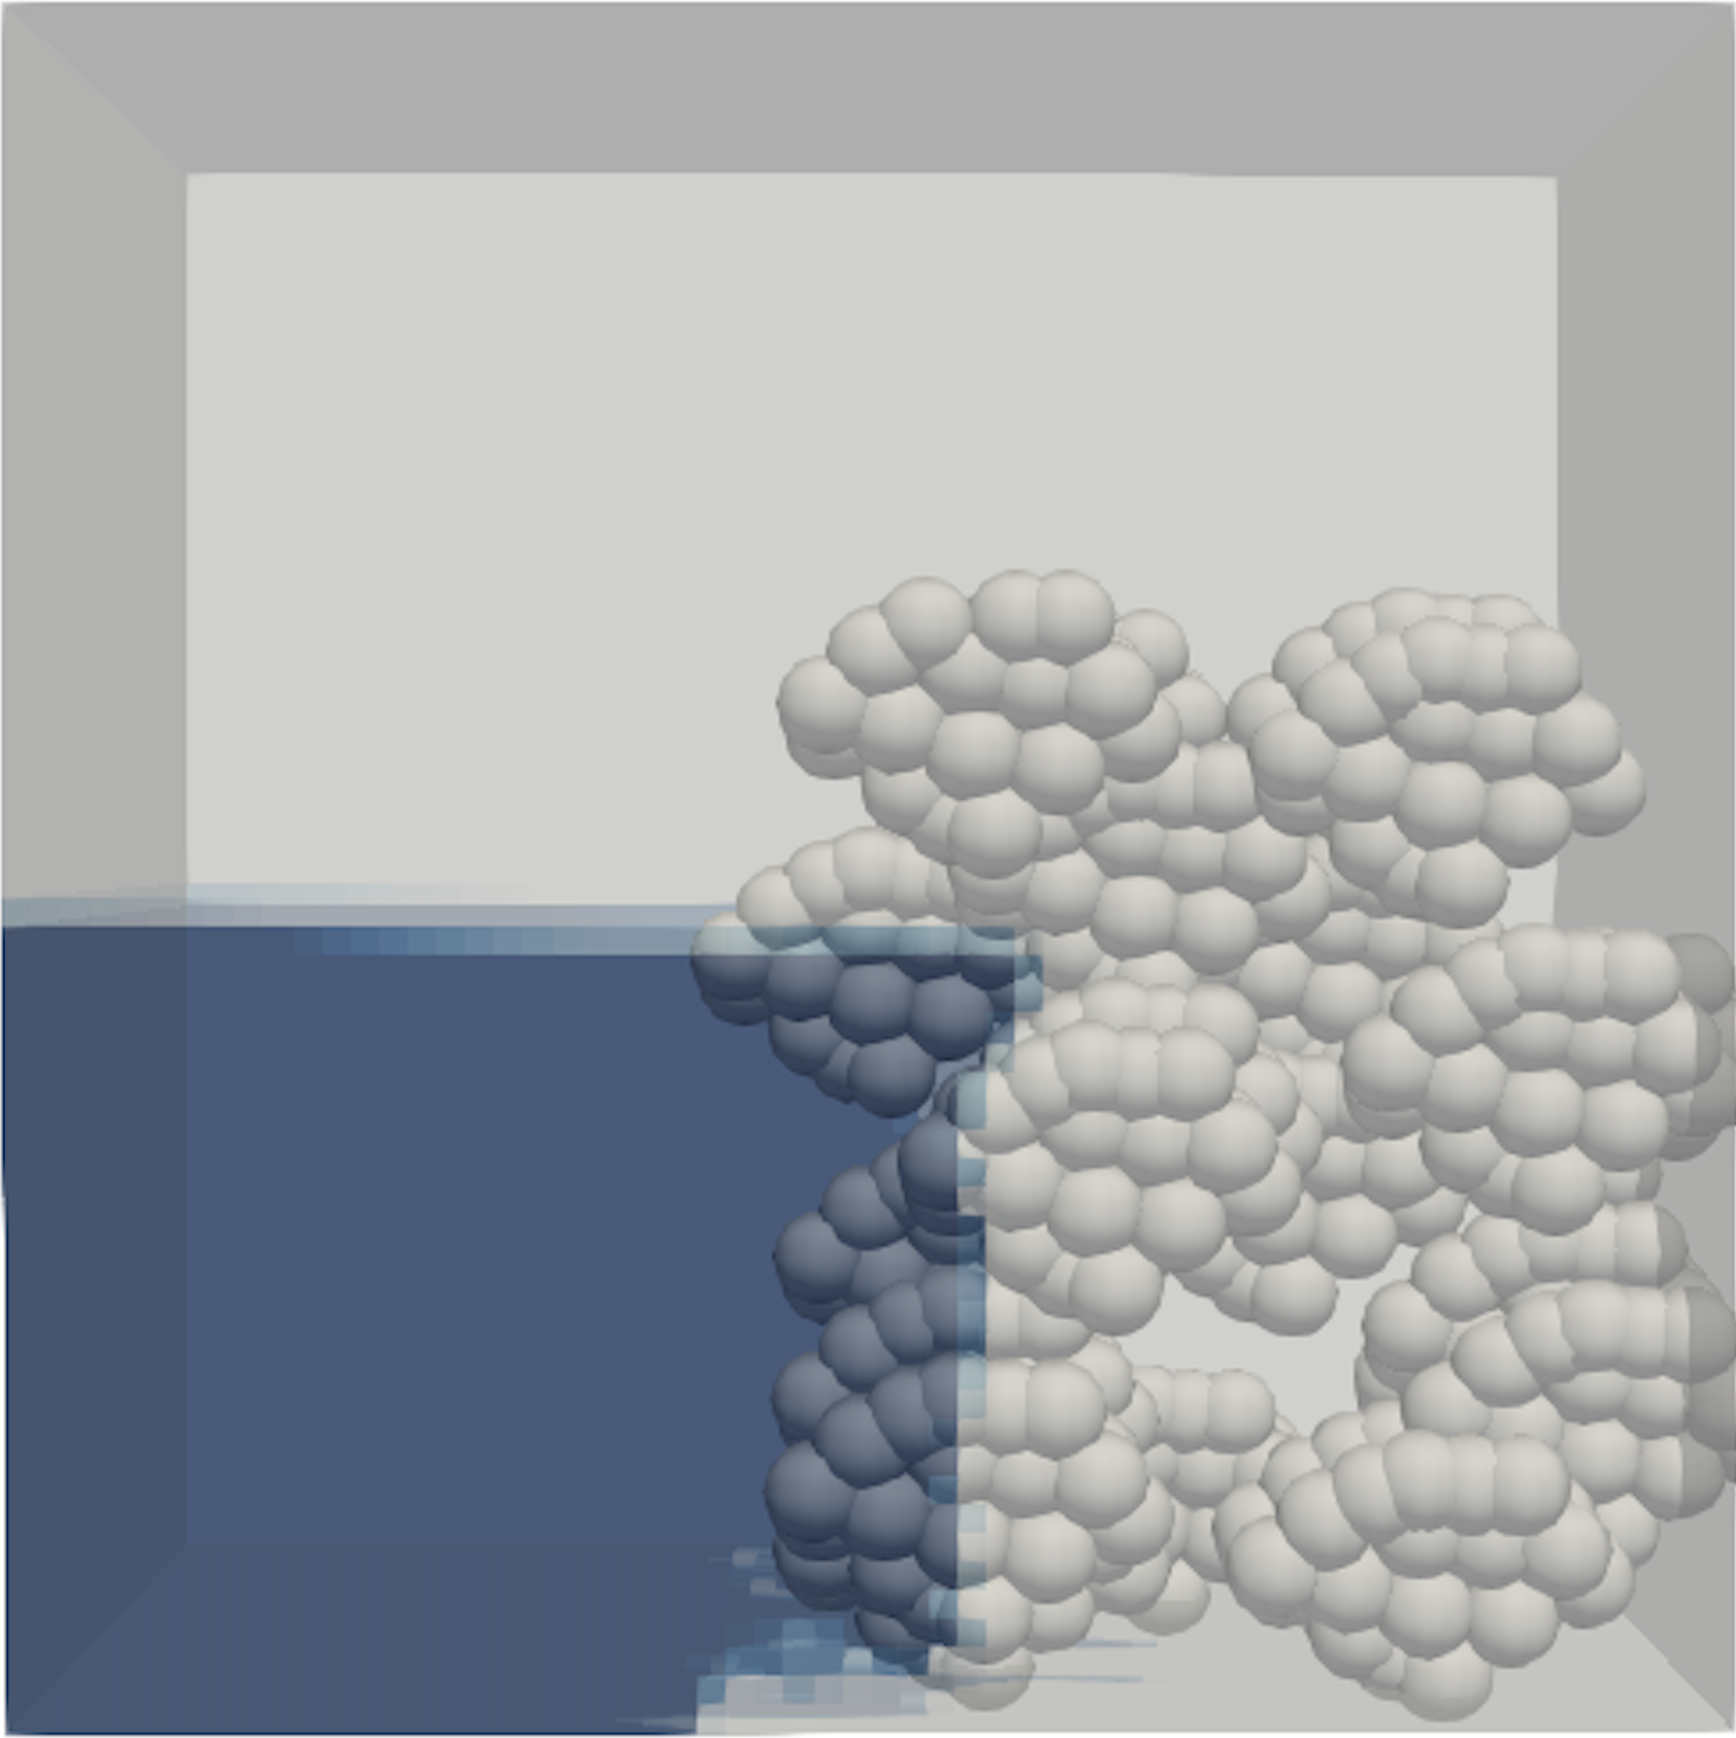
\includegraphics[width=\linewidth]{GWU_Thesis_Sarmakeeva/Images/chap4/landslide_1.png}
        \subcaption{0.05 sec}
    \end{minipage}%
    \hspace{0.05\textwidth}
    \begin{minipage}{.4\textwidth}
        \centering
        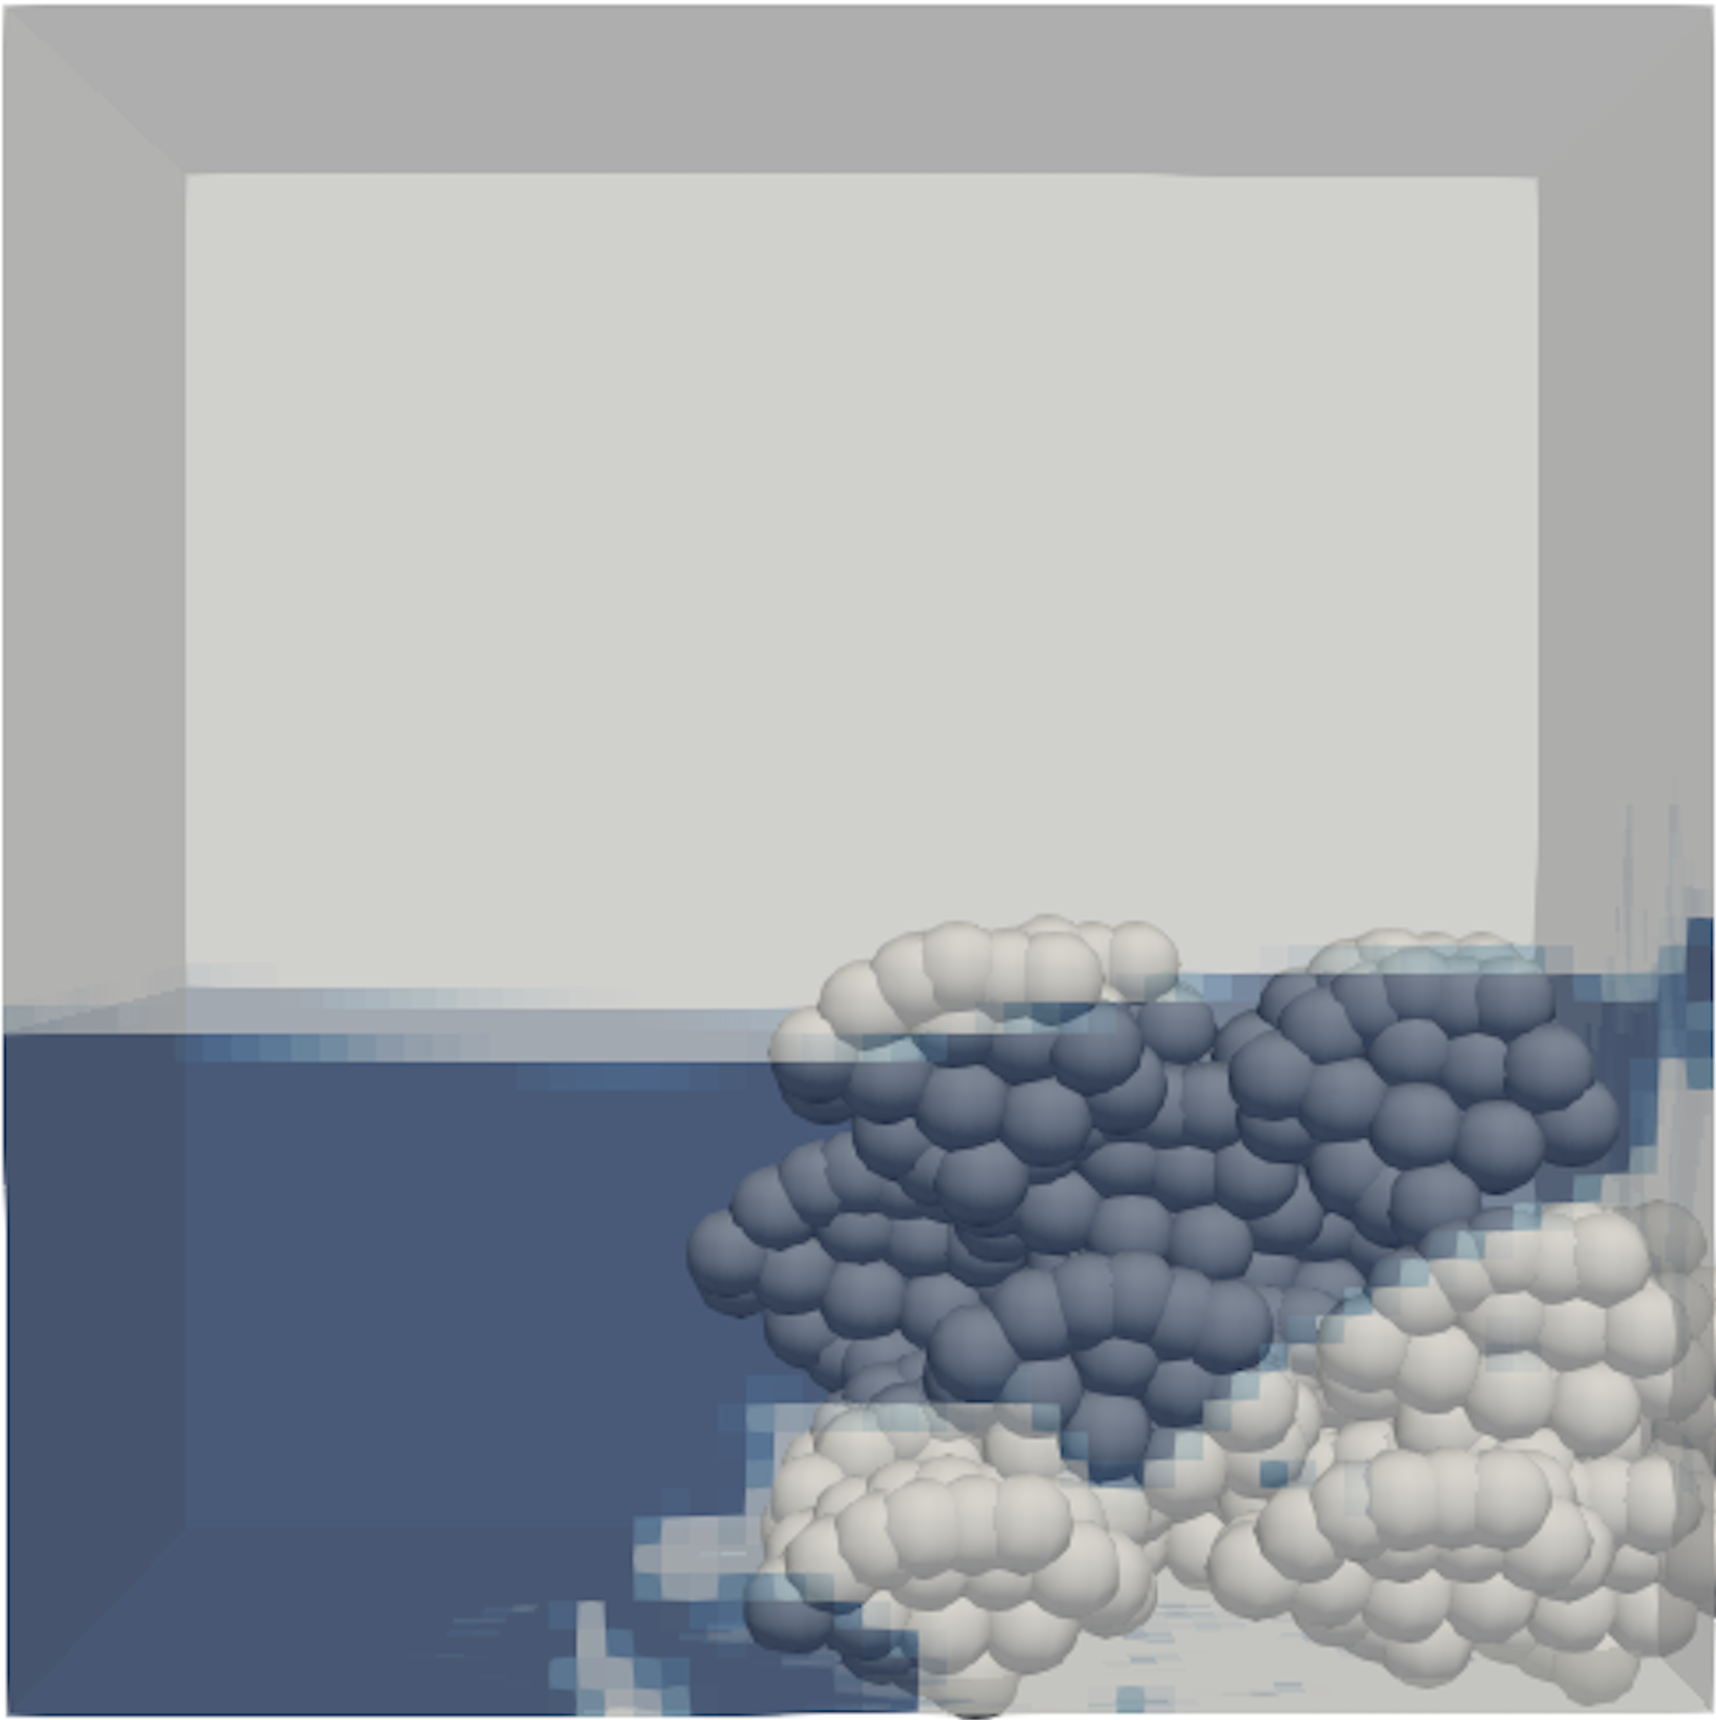
\includegraphics[width=\linewidth]{GWU_Thesis_Sarmakeeva/Images/chap4/landslide_2.png}
        \subcaption{0.1 sec}
    \end{minipage}
    \newline
    \begin{minipage}{.4\textwidth}
        \centering
        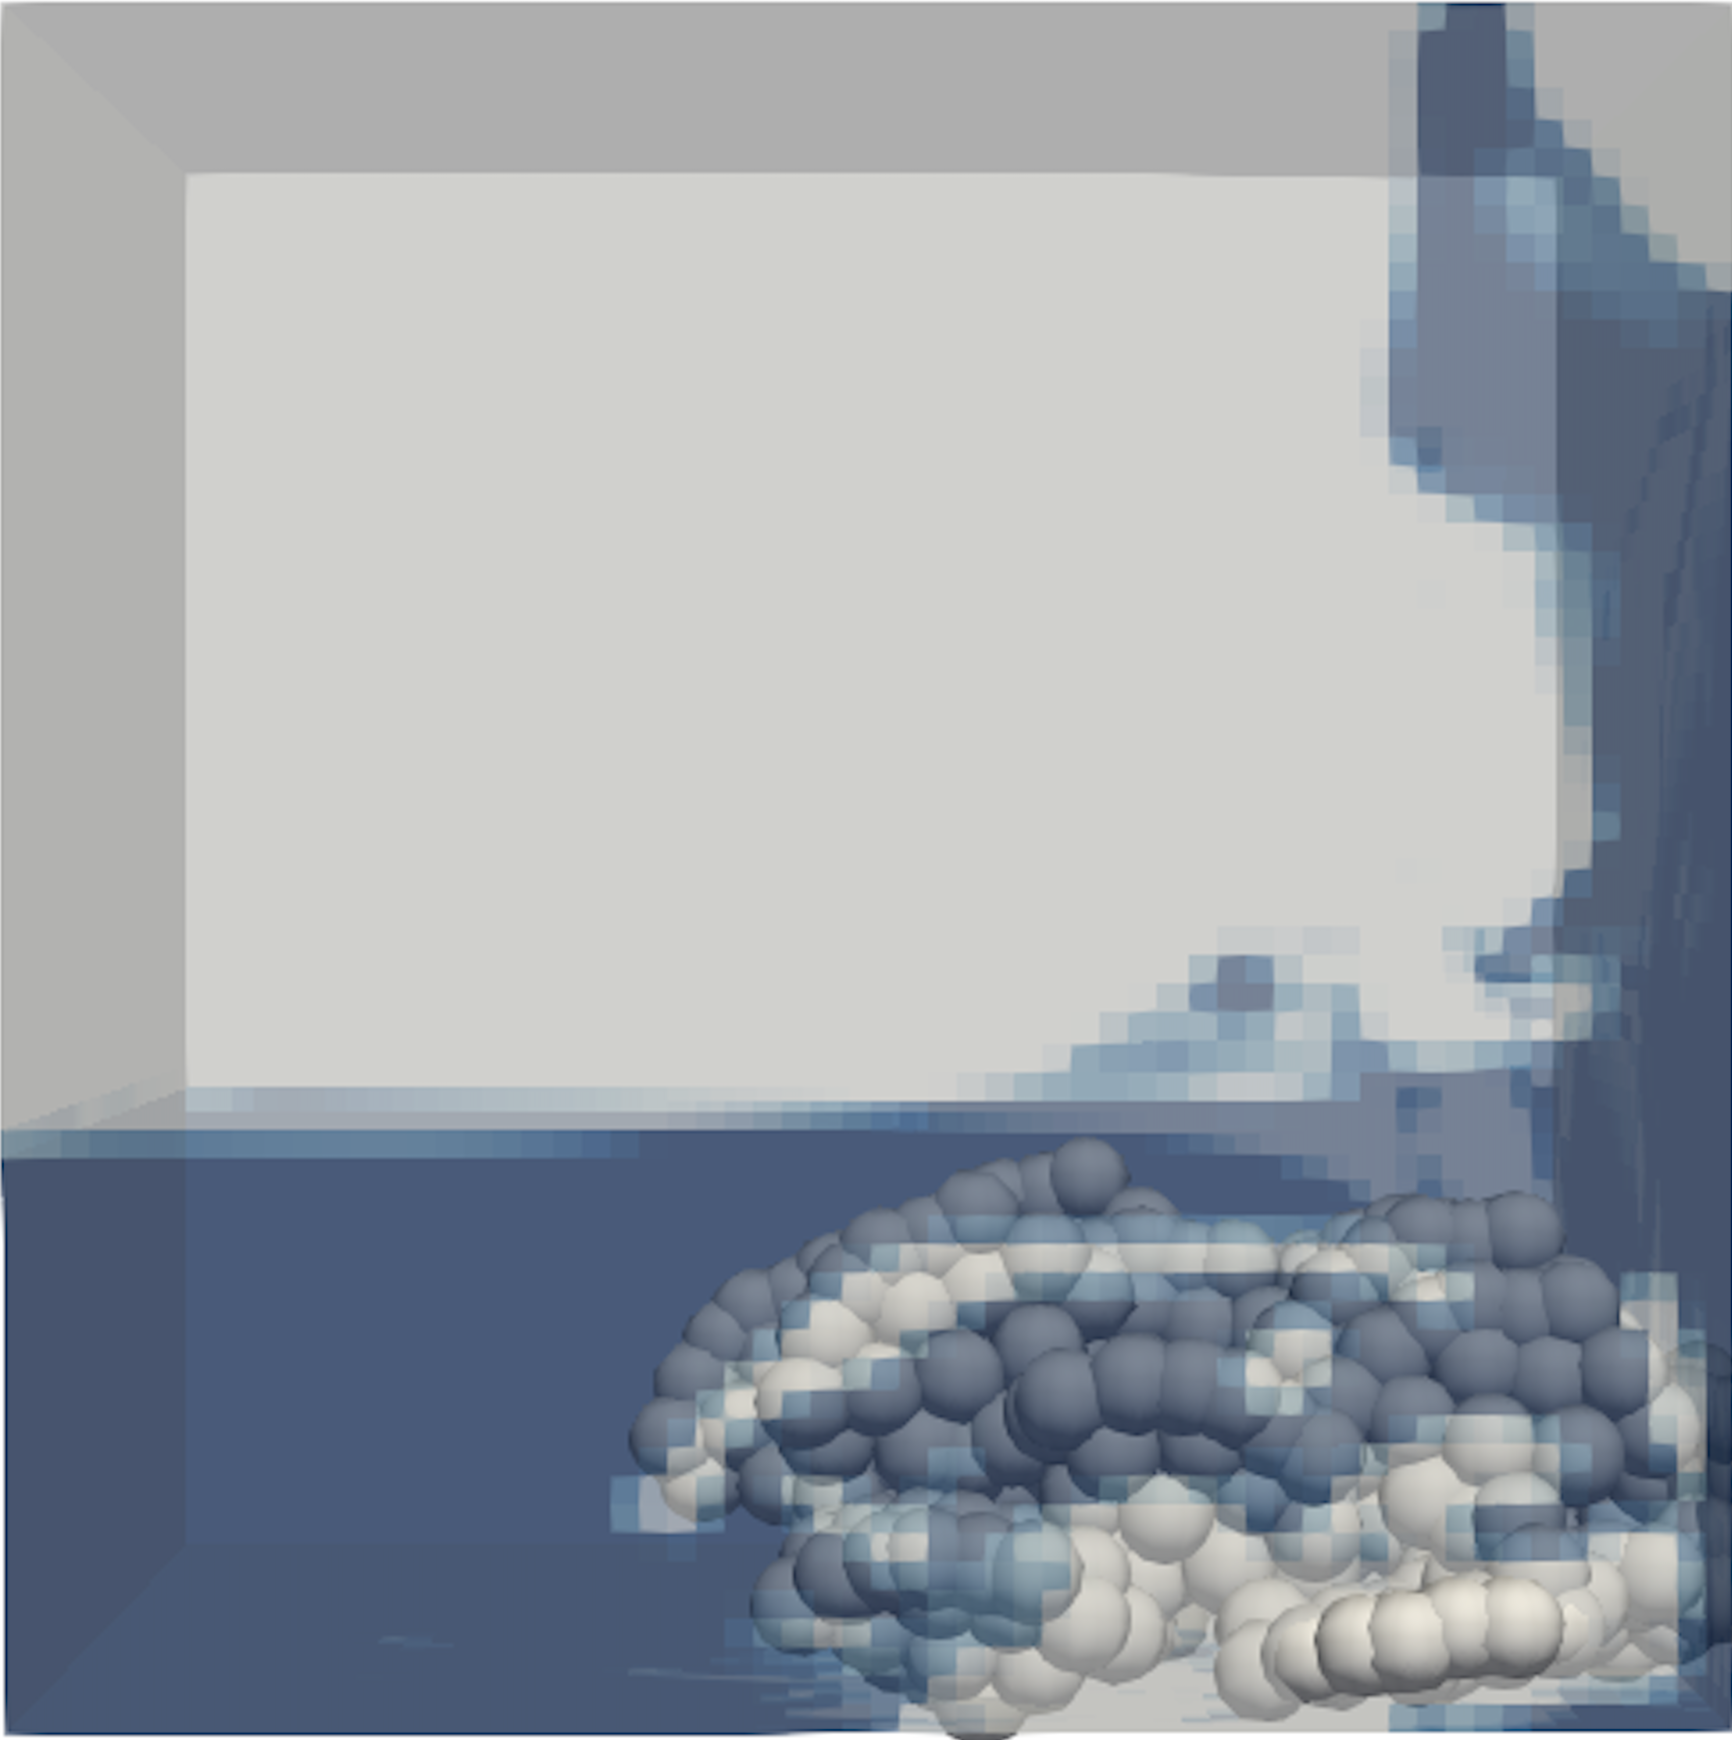
\includegraphics[width=\linewidth]{GWU_Thesis_Sarmakeeva/Images/chap4/landslide_3.png}
        \subcaption{0.15 sec}
    \end{minipage}%
    \hspace{0.05\textwidth}
    \begin{minipage}{.4\textwidth}
        \centering
        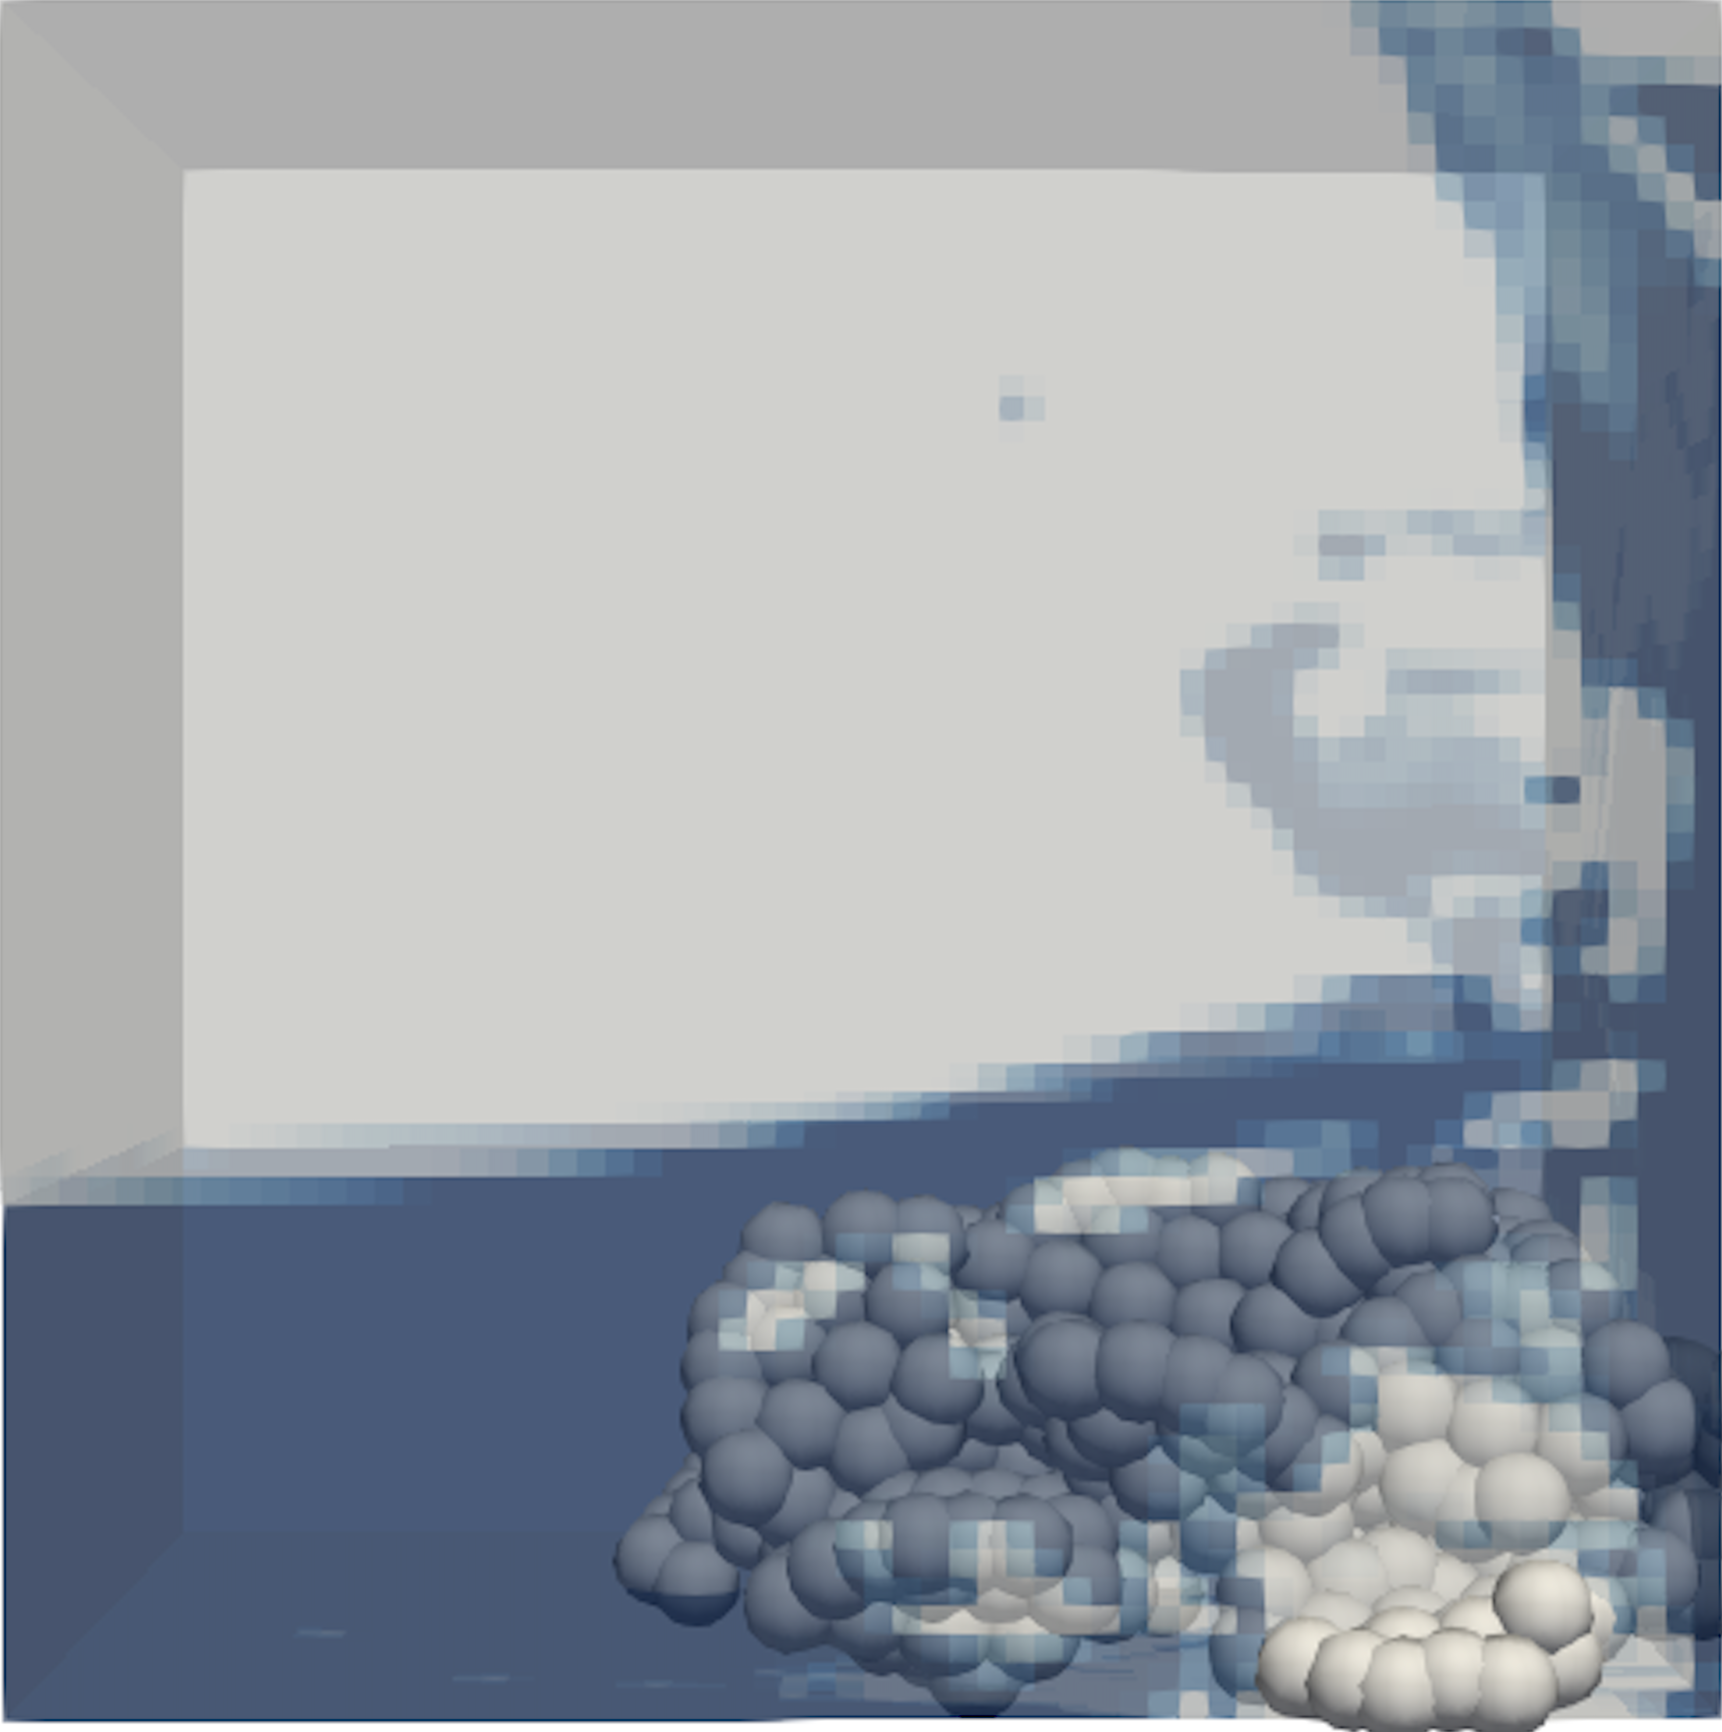
\includegraphics[width=\linewidth]{GWU_Thesis_Sarmakeeva/Images/chap4/landslide_4.png}
        \subcaption{0.2 sec}
    \end{minipage}
    \newline
    \begin{minipage}{.4\textwidth}
        \centering
        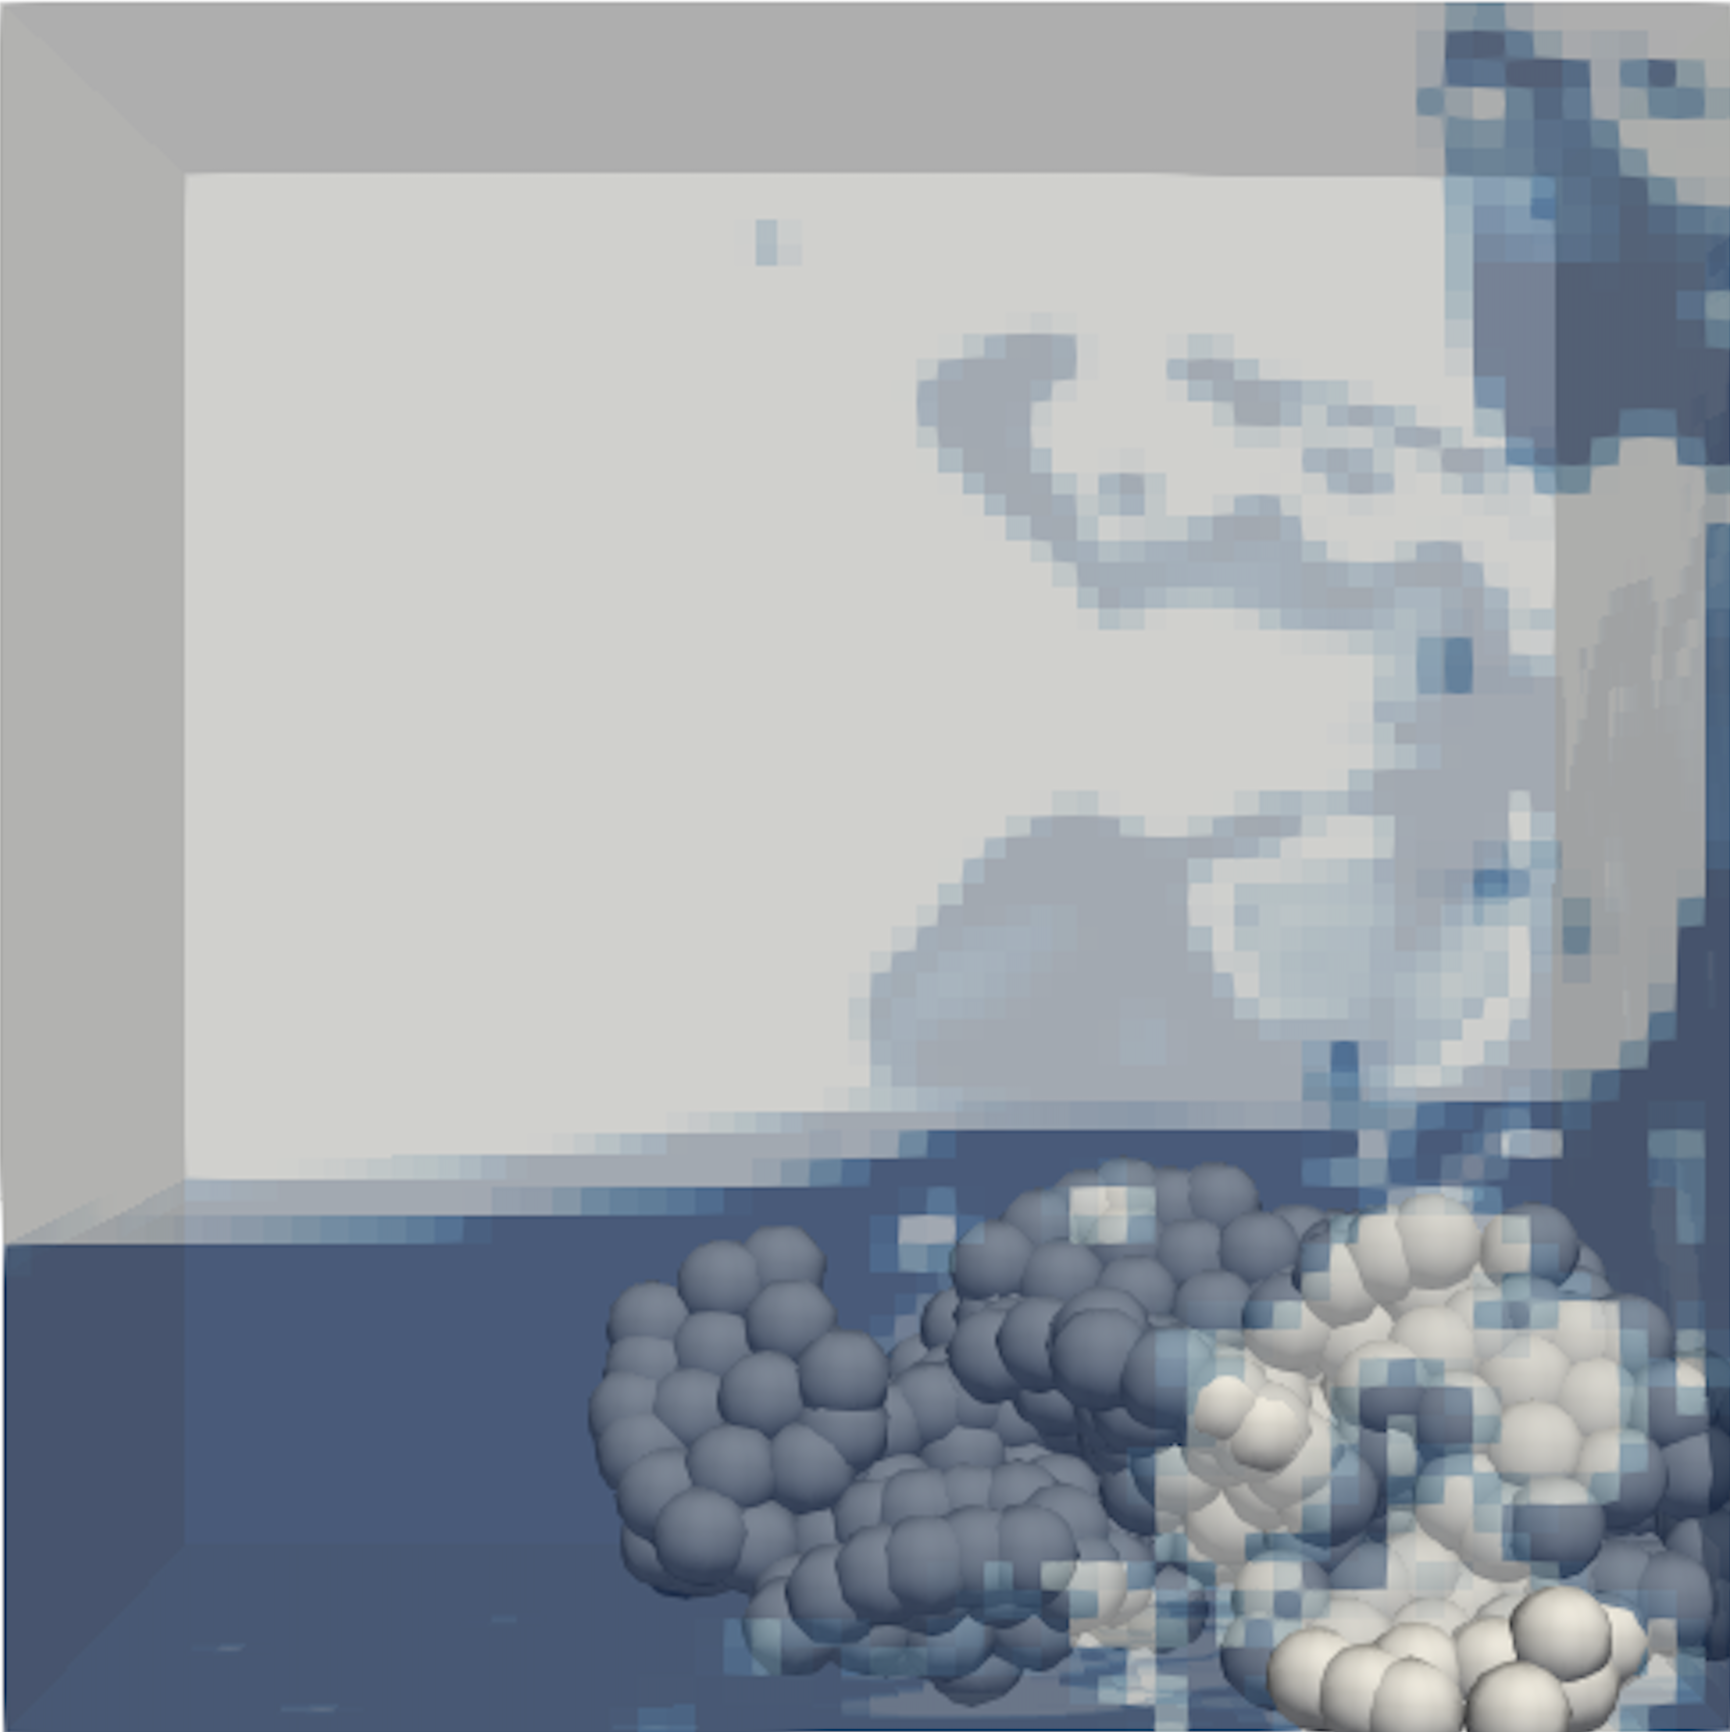
\includegraphics[width=\linewidth]{GWU_Thesis_Sarmakeeva/Images/chap4/landslide_5.png}
        \subcaption{0.25 sec}
    \end{minipage}%
    \hspace{0.06\textwidth}
    \begin{minipage}{.4\textwidth}
        \centering
        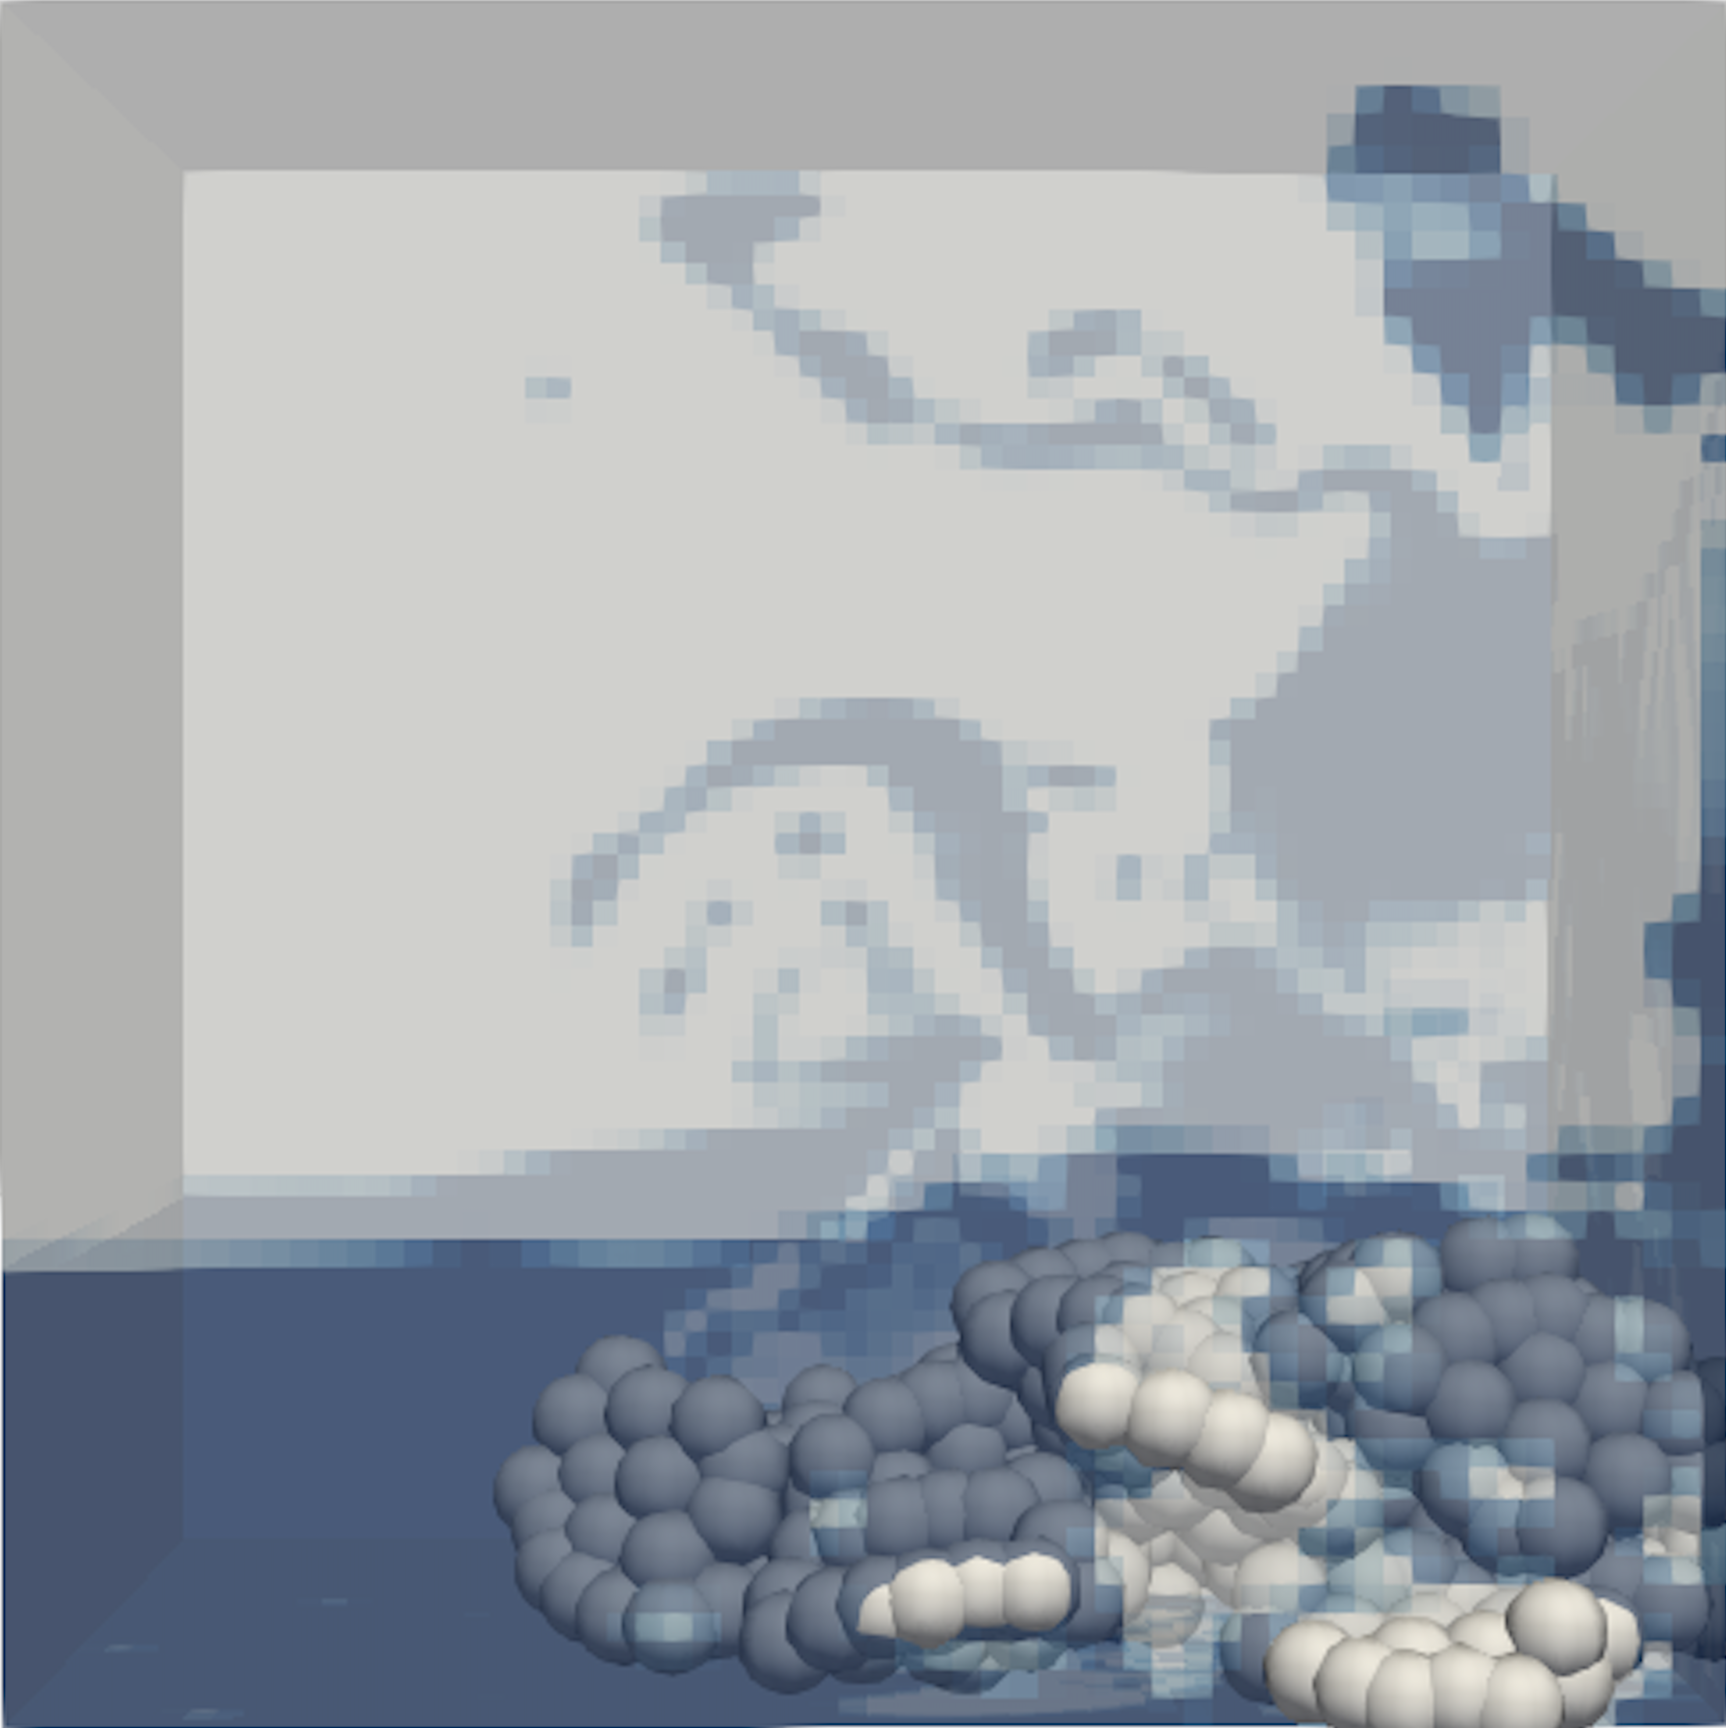
\includegraphics[width=\linewidth]{GWU_Thesis_Sarmakeeva/Images/chap4/landslide_6.png}
        \subcaption{0.3 sec}
    \end{minipage}
    \caption{Solid multi-spherical bodies interact with collapsing column of liquid: a) clumps placement b) clumps moving under gravity force c) clumps fully covered by body of fluid, fluid hits right boundary of the domain d) clumps continue to move under fluid and gravity forces e) fluid flow continue to develop f) developing fluid flow and solid bodies rotation.}
    \label{fig:two-phase_exp_clumps}
\end{figure}
Simulation run for $0.3$s with $\Delta t = 5e-5$. The clumps fall under gravity force in $z$-direction.

Figure \ref{fig:two-phase_exp_clumps} (a) shows clumps placement at $0.05$ sec; the water column begins to collapse under gravity. Some clumps are submerged, while others are still in contact with the air. In the second Figure \ref{fig:two-phase_exp_clumps} (b), the body of water is almost entirely covered with clumps and moving in the $z$ direction under the gravity force. In Figures \ref{fig:two-phase_exp_clumps} (c) - (f), the column of fluid has collapsed further. We can see a splash of water hit the right boundary of the box and the bodies rotating and settling at the bottom of the container. The interaction between the fluid and the spherical bodies continues to evolve, and the flow continues to develop.

Simulations on Figures \ref{fig:two-phase_exp} and \ref{fig:two-phase_exp_clumps} show that the created numerical algorithm could be used for large-scale computations with a larger number of particles. Code used for particle simulation \cite{LIGGGHTS} includes the possibility to use a number of clumps of different shapes, which also could approximate simulations better to real-world problems.

\begin{table}[H]
    \centering
    \caption{Computational time for multiple clump simulation.} \label{table4-chap4}
    \begin{tabular}{lr}
        \toprule
        \hline
       Number of processors     & Time (sec)\\
        \hline
        \midrule
        16 processors &  4500 sec \\
        32 processors &   2580 sec\\
        64 processors &   1320 sec\\
                                \hline
        \bottomrule
     \end{tabular}
\end{table}
Table \ref{table4-chap4} shows computational times for a multiple clump simulation with varying numbers of processors. The results show that the simulation benefits from parallel processing, as evidenced by the decrease in computational time when the number of processors is doubled. When increasing the number of processors from 16 to 32, the computational time decreases from 4500 seconds to 2580 seconds. This represents a reduction of approximately 42.7\%. Further, increasing the number of processors to 64 reduces the time to 1320 seconds, about 49.2\% less than the time taken with 32 processors and approximately 70.7\% less than the time with 16 processors. These results show the benefits of parallel computation for the developed solver.

\section{Discussion}

%The initial goal of this work was to develop a tool that could be used for the simulation of landslides in coastal areas. To do so, we need to figure out methods suitable for this type of problem based on open-source code, then implement, verify, validate, and then test it. This is a nontrivial task and requires significant work. Validation and verification showed that the solver works as we suppose. Based on that, we run simulations testing the solver in more detail. We tested on bouncing body simulation, which showed stable results. Then we ran the simulation with multispherical bodies interaction and fluid with a developed solver, showing that it could handle complex interactions between solid and liquid phases effectively and the dynamics of multiple solid bodies. This capability is important for accurately simulating real-world scenarios such as landslides, sediment transport, and other particulate flow problems. The solver can manage geometrical complexities, as seen in the last simulation in Figure \ref{fig:two-phase_exp_clumps}. It can track the motion and interaction of bodies with non-uniform shapes through the fluid, which involves complex boundary conditions and potentially non-linear material behavior. The solver is effective for parallel computations by the decreased computation times with increased processor counts, as shown in Table \ref{table4-chap4}. Documentation for the solver is available online \ref{sarmakeeva_multiphaseIB}, as well as detailed documentation.

The primary objective of this study was to create a robust simulation tool tailored for analyzing landslide phenomena in coastal environments. This endeavor required identifying and implementing suitable methods and leveraging open-source code as a foundational framework. The complexity of this task necessitated a comprehensive approach encompassing implementation, verification, validation, and extensive testing.

Our verification and validation processes confirmed that the solver operates in line with our theoretical expectations. Subsequent to this, we embarked on a series of intricate simulations to examine the solver's capabilities further. Initial tests involving the simulation of a bouncing body yielded stable outcomes, affirming the solver's reliability. Progressing further, we conducted simulations incorporating multispherical bodies interacting within a fluid using our developed solver. These tests demonstrated the solver's adeptness in managing complicated interactions between solid and liquid phases. This proficiency is critical for the accurate representation of real-world phenomena such as landslides, sediment transport, and other scenarios involving particulate flows.

A significant aspect of our solver is its ability to handle geometric complexities. This is evidenced in our simulations (see Figure \ref{fig:two-phase_exp_clumps}), where the solver tracked the motion and interaction of irregularly shaped bodies within the fluid. Given the complex boundary conditions and potential non-linear material behavior encountered in such simulations, this capability is crucial.

Moreover, our solver exhibits excellent scalability and efficiency in parallel computing environments. We observed a notable reduction in computation times with the increase in processor counts, as detailed in Table \ref{table4-chap4}. This scalability is particularly beneficial for handling the computationally intensive tasks associated with fluid-solid interaction simulations.

Documentation of our solver, including its theoretical foundations, implementation details, and usage guidelines, is accessible online (see \ref{sarmakeeva_multiphaseIB}). This resource is intended to assist researchers and practitioners in adopting and adapting our tool for their specific needs, thereby contributing to the broader scientific community's understanding and management of complex fluid-solid interactions.

 





